%%%%%%%%%%%%%%%%%%%%%%%%%%%%%%%%%%%%%%%%%%%%%%%%%%%%%%%%%%%%%%%%%%%%
%% I, the copyright holder of this work, release this work into the
%% public domain. This applies worldwide. In some countries this may
%% not be legally possible; if so: I grant anyone the right to use
%% this work for any purpose, without any conditions, unless such
%% conditions are required by law.
%%%%%%%%%%%%%%%%%%%%%%%%%%%%%%%%%%%%%%%%%%%%%%%%%%%%%%%%%%%%%%%%%%%%

\documentclass[
  printed,     %% The `digital` option enables the default options for the
               %% digital version of a~document. Replace with `printed`
               %% to enable the default options for the printed version
               %% of a~document.
  color,       %% Uncomment these lines (by removing the %% at the
               %% beginning) to use color in the printed version of your
               %% document
  oneside,     %% The `oneside` option enables one-sided typesetting,
               %% which is preferred if you are only going to submit a
               %% digital version of your thesis. Replace with `twoside`
               %% for double-sided typesetting if you are planning to
               %% also print your thesis. For double-sided typesetting,
               %% use at least 120 g/m² paper to prevent show-through.
  nosansbold,  %% The `nosansbold` option prevents the use of the
               %% sans-serif type face for bold text. Replace with
               %% `sansbold` to use sans-serif type face for bold text.
  nocolorbold, %% The `nocolorbold` option disables the usage of the
               %% blue color for bold text, instead using black. Replace
               %% with `colorbold` to use blue for bold text.
  nolof,         %% The `lof` option prints the List of Figures. Replace
               %% with `nolof` to hide the List of Figures.
  nolot,         %% The `lot` option prints the List of Tables. Replace
               %% with `nolot` to hide the List of Tables.
]{fithesis4}
%% The following section sets up the locales used in the thesis.
\usepackage[resetfonts]{cmap} %% We need to load the T2A font encoding
\usepackage[T1,T2A]{fontenc}  %% to use the Cyrillic fonts with Russian texts.
\usepackage[
  main=english, %% By using `czech` or `slovak` as the main locale
                %% instead of `english`, you can typeset the thesis
                %% in either Czech or Slovak, respectively.
  english, german, russian, czech, slovak %% The additional keys allow
]{babel}        %% foreign texts to be typeset as follows:
%%
%%   \begin{otherlanguage}{german}  ... \end{otherlanguage}
%%   \begin{otherlanguage}{russian} ... \end{otherlanguage}
%%   \begin{otherlanguage}{czech}   ... \end{otherlanguage}
%%   \begin{otherlanguage}{slovak}  ... \end{otherlanguage}
%%
%% For non-Latin scripts, it may be necessary to load additional
%% fonts:
\usepackage{paratype}
%%
%% The following section sets up the metadata of the thesis.
\thesissetup{
    date        = 2023/05/15,
    university  = mu,
    faculty     = fi,
    type        = mgr,
    department  = Department of Computer Systems and Communications,
    author      = Bc. Lukáš Perina,
    gender      = m,
    advisor     = {RNDr. Milan Čermák, Ph.D.},
    title       = {Automated detection of modified network traffic captures},
    TeXtitle    = {Automated detection of modified network traffic captures},
    keywords    = {computer networks, protocols, packet capture, forensic analysis, modification detection methods, network traffic},
    TeXkeywords = {computer networks, protocols, packet capture, forensic analysis, modification detection methods, network traffic},
    abstract    = {%
      This master's thesis aims to develop an automated detection application that would enable security professionals and forensic analysts to verify the originality of the packet trace capture files. The thesis introduces the reader to the network traffic capture processing with the currently available tools and protocols. This introduction is crucial in order to understand the context of different terms and relationships between the structures and protocol behavior. Subsequently, the modification of captured data is analyzed, the tools commonly used for this task are presented, and the associated risks and impact of such actions are discussed. Detection method approaches are described and presented as a~base for further research on modification detection. Even though these are often representative of live traffic scanning, the strategies still apply for the packet capture analysis as well. The practical part of this thesis presents the proposed solution as an application that incorporates multiple modules and provides packet capture analysis with multiple detection algorithms implemented. The application uses these algorithms to analyze packet capture files and calculate the resulting probability of packet capture manipulation. From a dataset generated in order to verify the application functionality, an average of 56.82\% modification probability was observed.
    },
    thanks      = {%
      I would like to express my deepest gratitude to my thesis advisor, RNDr. Milan Čermák, Ph.D., for his unwavering support, expert guidance, and mentorship throughout my research journey. His expert skills, constructive criticism, and valuable insights have greatly impacted the quality and scope of my work. I am thankful for his professional attitude and willingness to assist me in the toughest times.
    },
    bib         = bibliography.bib,
    %% Remove the following line to use the JVS 2018 faculty logo.
    facultyLogo = fithesis-fi,
}
\usepackage{makeidx}      %% The `makeidx` package contains
\makeindex                %% helper commands for index typesetting.
%% These additional packages are used within the document:
\usepackage{paralist} %% Compact list environments
\usepackage{amsmath}  %% Mathematics
\usepackage{amsthm}
\usepackage{amsfonts}
\usepackage{url}      %% Hyperlinks
\usepackage{markdown} %% Lightweight markup
\usepackage{listings} %% Source code highlighting
\usepackage{comment}
\usepackage{enumitem}
\usepackage{adjustbox}
\usepackage{fancyvrb}
\usepackage{booktabs}
\usepackage{dirtree}
\lstset{
  basicstyle      = \ttfamily,
  identifierstyle = \color{black},
  keywordstyle    = \color{blue},
  keywordstyle    = {[2]\color{cyan}},
  keywordstyle    = {[3]\color{olive}},
  stringstyle     = \color{teal},
  commentstyle    = \itshape\color{magenta},
  breaklines      = true,
}
\usepackage{floatrow} %% Putting captions above tables
\floatsetup[table]{capposition=top}
\usepackage[babel]{csquotes} %% Context-sensitive quotation marks
\usepackage{minted}

\begin{document}

\chapter{Introduction}

The purpose of this thesis is to research the topic of a network traffic capture analysis, the possibilities to manipulate the packet captures, and to design and implement an application that will be able to detect modifications made to the packet captures. Currently, the research on this topic is not widely spread because most topics talk about live traffic scanning~\cite{ABBASI202119}. This work concentrates on network packet trace analysis and aims to develop an application that will attempt to detect changes made to these offline packet traces.

The modifications made to the network packet traces might be done by the attacker in order to hide the traces left after his malicious act. Since the packet captures could be used as evidence during a~forensic analysis, these files must be protected, and their integrity has to be ensured. There also needs to be a~way to determine the originality of the file and to ensure that the file was not modified. This is where the proposed solution might bring more light to this topic. Detecting such changes is not an easy task, and the detection might be influenced by various properties. These might range from the skill of an attacker modifying the packet trace to the complexity of the network and the nonstandard behavior of some of the network components.

The importance of protecting the network packet capture integrity is escalated by the fact that the ever-growing number of networks is acting as a~bigger and bigger target for attackers and malicious acts. These might include personal information stealing or targeting specific networks in order to gain access to network resources.

The first part of the work in Chapter \ref{chap:ntc} introduces the reader to the world of network traffic capture. It also describes available monitoring strategies, as well as the challenges and underlying network protocols, which are deeply analyzed. The following Chapter \ref{chap:modif} analyses the possibilities to modify the network captures traces, the tools available to do so, and the associated risks with such modifications.
Chapter \ref{chap:mdm} discusses modification detection methods. The description of these methods comes from live traffic analysis. Still, their core principle also applies to packet capture trace analysis, and they form a~great knowledge base for further development. In Chapter \ref{chap:desimp}, the design and implementation of the proposed application are discussed. The application's requirements, architecture, and structure are described in detail. The proposed detection methods are also described in this Chapter. Finally, Chapter \ref{chap:testing} describes how application testing was conducted, with the tests performed and results discussed at the end of this Chapter.





\newpage
\chapter{Network traffic capture}
\label{chap:ntc}

This chapter will discuss the fundamentals of network traffic capture, which are essential for the forensic analysis of digital data. Capturing network packets can be a~challenging and complex task since the operating system may provide inaccurate information, and malware can interfere with the capture process directly~\cite{Messier2017-fz}. It is important to understand that even if we call it packet capture, what we are really capturing are \textit{frames}. While there was a~time when only specialized hardware and network interfaces were capable of capturing packets, nowadays, nearly all network interfaces and devices with a~common operating system can perform this task.


\section{Capturing network data}

The motivation behind network monitoring is that it brings substantial benefits and is useful while maintaining the network. These can be, for example troubleshooting various problems and anomalies, accounting, and security reasons. It is an essential tool used to troubleshoot and resolve connection problems, which in the current world of connected devices could cause serious trouble or even damage. Capturing and monitoring Internet traffic is the process of observing the flow of data between two devices on a~given network. This gives us the ability to see what exactly is going on and to potentially discover bottlenecks, malicious activity, and even other network-related problems. Monitoring of traffic involves observation of the flow of data on a~given network using specialized tools that allow us to listen to the data that are being transmitted. For these observations, it is a~necessity to use specialized software and sometimes even hardware.

When performing the network capture, there are two main schemes of capturing the data -- passive monitoring and active monitoring. Lately, there has been ongoing research on a~hybrid type of monitoring~\cite{261437}, which combines active and passive into one.


\paragraph{Active monitoring} operates on a~unique principle~\cite{landfeldt2000case}. By inserting probes into the network, it is able to monitor and gather information about a~given network, like bandwidth, round trip delays, or network speed. Bottlenecks can be detected by using a~back-to-back technique or packet-pair probing. To estimate the bandwidth available, the active monitoring generates traffic and uses ICMP echo packets to get this information. This type of monitoring is considered highly accurate. However, it competes for network resources. This huge disadvantage means it has a~high impact on the network and is therefore not recommended for crucial networks which can be negatively affected.

\paragraph{Passive monitoring} is the most common type of network traffic capture. It overcomes the disadvantages of active schemes by passively monitoring streams of data~\cite{Messier2017-fz}. To do this effectively, they infer the current network status and the information about the network in such a~way that they do not need to introduce new traffic to the network in order to gather those pieces of information. Passive monitoring is often done through SPAN port or via network tap:

\begin{itemize}
    \item a~\textbf{TAP(Test Access Point)} refers to a~hardware device that is used to monitor network traffic passively. A~TAP is inserted between two network devices, such as a~router and a~switch, to essentially intercept and copy any traffic flowing through them. It copies all traffic passing through, regardless of the port that the traffic is coming from or going to. This makes it a~complete monitoring solution. TAPs are used in situations where it is important to capture all network traffic for security reasons or compliance auditing.
    \item a~\textbf{SPAN(Switch Port Analyzer)} or port spanning is a~technique used to capture network traffic on a~network device called a~switch. In port spanning, the switch is configured with a~SPAN port in such a~way that it copies packets that are transmitted over a~particular port or set of ports and sends them to a~designated port called a~SPAN port or mirroring port. This port is connected to a~device such as a~network analyzer or packet capture tool in order to capture the network data.
\end{itemize}

\subsection{Network packets}

To capture the traffic, we monitor the network and save each packet that flows through it. The network packet represents a~chunk of data sent over a~network between two devices at either end of the communication channel~\cite{PacketMD39:online}. There are generally two main components, user data and control information. The former is commonly known as \textit{payload} and carries the data from one device to another. The latter is the information critical for delivering the payload. This consists of network addresses, sequencing information, and error detection codes. This information is found in the packet's \textit{header} and its \textit{footer}. 

Control information should always contain specific information based on what type of packet is currently used. There are many packet layers, each containing information specific to that layer. Some of the most common network packet layers are the following:

\begin{itemize}
    \item Ethernet layer: specifies electrical and optical properties,
    \item IP layer: used for communication between different networks, including the Internet,
    \item TCP layer: used for reliable data transmission between devices over the networks.
\end{itemize}

However, considering the nature of the internet and the everlasting continuous exponential growth of demand for new applications, there are many more types used in networking depending on the application used.

The TCP/IP model, as shown in Figure \ref{fig:tcpipmodel}, consists of 4 layers, compared to ISO/OSI with seven layers. The strength of the ISO/OSI model is, in fact, the model itself, which is extraordinarily useful when learning about computer networks~\cite{10.5555/2584507}. On the other hand, TCP/IP model helps us understand the protocols more directly. The protocols are an important part of this thesis, and this model provides a~clear representation of where they belong. Attackers may use this knowledge to hide malicious data based on the network layer protocol.

\begin{figure}[h]
  \begin{center}
    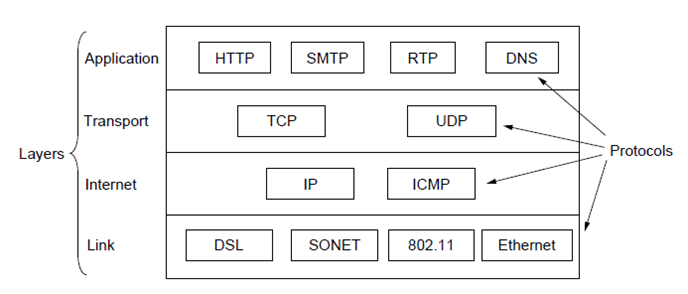
\includegraphics[width=1\textwidth]{images/tcpip_new.png}
  \end{center}
  \caption{The TCP/IP model~\cite{10.5555/2584507}}
  \label{fig:tcpipmodel}
\end{figure}

\newpage

\begin{itemize}
    \item \textbf{The Link Layer:} TCP/IP model does not directly mention the physical layer. Instead, it now concentrates on how to send messages directly between computers using either Ethernet or 802.11 protocols on the \textbf{Link layer}.

    \item \textbf{The Internet Layer:} Holding the whole architecture together, the Internet Layer of the TCP/IP model roughly corresponds to ISO/OSI network layer. Its main purpose is to allow hosts to send packets into any network on the Internet and have them travel independently on each other. This layer defines an official packet format called IP (Internet Protocol) and a~companion protocol called ICMP (Internet Control Message Protocol) that cooperates directly with the IP. Together, their job is to deliver packets to the destination.

    \item \textbf{The Transport Layer} is the layer above the Internet Layer in the TCP/IP model. Just as in ISO/OSI model, it is designed to allow two devices to communicate. There have been two major protocols that were defined in this layer. These are TCP (Transmission Control Protocol) and UDP (User Datagram Protocol).

    \item \textbf{The Application Layer:} TCP/IP model's highest layer is called the Application Layer. It is responsible for providing clear communication services directly to the application. It provides a~way for applications to access network services and establish direct communication with other applications on remote devices called hosts. Communication protocols such as HTTP, FTP, DNS, or Telnet are all implemented on this layer. The Application Layer also provides a~way to authenticate, authorize and encrypt application data to ensure secure communication.
\end{itemize}


\section{Common packet capture file formats}

When capturing network data, knowing what we want to capture is important. We use specialized file formats to store the captured packets, which are essential for this thesis. The most common are \textbf{PCAP} and \textbf{PCAPNG}. These formats are both part of LibpcapFileFormat and are also used by many monitoring tools that will be described later.

\subsection{LibpcapFileFormat}

The LibpcapFileFormat~\cite{LibpcapF59:online}~\cite{LibpcapF97:online} is a~file format that is the main file format used by many networking tools, including Wireshark~\cite{Wireshar89:online} and TShark\footnote{\url{https://linux.die.net/man/1/tshark}}. It represents a~very simple file format for saving captured network data and is a~standard of network capturing in UNIX operating systems. Later, the Windows operating system adopted libpcap under the name WinPcap. WinPcap\footnote{\url{https://www.winpcap.org/}} is, however, currently obsolete, replaced by npcap\footnote{\url{https://npcap.com/}}.

\subsubsection{PCAP}

The proposed file extension for libpcap files is PCAP, and it stands for \enquote{Packet Capture}. This file format has been unchanged since 1998, and it consists of the following data:

\begin{itemize}
    \item \textbf{Global header:} Global information about the PCAP file, such as the magic number used to determine the file format itself and the byte order, timezone, and version information.
\end{itemize}

After the global header, which contains information about the file itself, there is a~list of packets, one by one, always starting with a~header and followed by data. The rest of the PCAP file then looks like this:

\begin{itemize}
    \item \textbf{Packet Header:} Each captured packet starts with header. The packet header contains the timestamp when the packet was captured in UNIX time. It also contains microseconds when this packet was captured, the number of bytes, and the length of the packet.
    \item \textbf{Packet data:} Data that were transmitted over the network will immediately follow the packet header.
\end{itemize}

PCAP file format is still commonly used. However, it is slowly being replaced by more modern file formats. One of the file formats that is worth mentioning is PCAPNG.

\subsection{PcapNG}

The PcapNG file format~\cite{PcapNg85:online}, which stands for PCAP Next Generation, is a~newer capture file format designed to overcome multiple limitations of the original PCAP. These limitations include the inability to store packets with different link layers and many others. It is also more flexible, supporting advanced features such as capturing metadata, custom block types, and multiple interfaces in a~single file. It also has better support for timestamp precision, which is one billionth of a~second, compared to Pcap with just one-millionth of a~second. It allows for comments, annotations, and other data to be attached to packets. Data structures are designed for storing metadata such as hostnames, even encryption keys, and much more. 

It became the default save-file format for Wireshark in 2012, which has been the main reason many people and companies switched over to it. Despite this fact, PCAP is still more widely used across many industries.

\section{Monitoring tools}

To monitor the network traffic, there are currently a~number of tools that one can use in order to do so efficiently. The most important thing to keep in mind is that a~computer with a~network card and operating system like Windows or Linux is often enough to do basic network monitoring. The applications that were the most useful for this thesis will now be covered.

The differences often consist not of the features available but rather usage characteristics. Command line tools are mostly used for scripting and automatization, while GUI-based tools can provide us with clearer info and an intuitive user interface. Ultimately, it comes down to what one prefers and what kind of usage and outcome one prefers from a~given application.

\subsection{Wireshark}

One of the most popular network monitoring software out there is surely Wireshark~\cite{Wireshar89:online}. It is used to analyze networks and the protocols that are being used. It can monitor what exactly is happening with a~straightforward and intuitive GUI. The project of developing Wireshark started in 1998 and has since been considered standard across many industry levels. It offers features like deep inspection of protocols, live capture, and offline analysis or packet browser. Multiple display filters are a~crucial feature, and Wireshark even allows one to read and write many different file formats, including PCAP and PCAPNG, which were discussed earlier. 

It supports reading live data from either Ethernet or IEEE 802.11 and many more. Wireshark GUI, shown in Figure \ref{fig:wireshark}, comes with coloring rules that will, at first glance, show the type of packet on an intuitive basis. Being free and open-source software means that anyone can tinker with it and use it to troubleshoot the problems on his network. That is why Wireshark is widely used by network administrators, security professionals, developers, and, last but not least, researchers to develop new network protocols. Earlier versions also offered a~packet editor, but this functionality has since been discontinued. Wireshark is an essential tool that is well-known among network professionals because of its industry-leading features. It provides a~simple user interface and helps explore traffic on the network with outstanding capabilities.

\begin{figure}[h]
  \begin{center}
    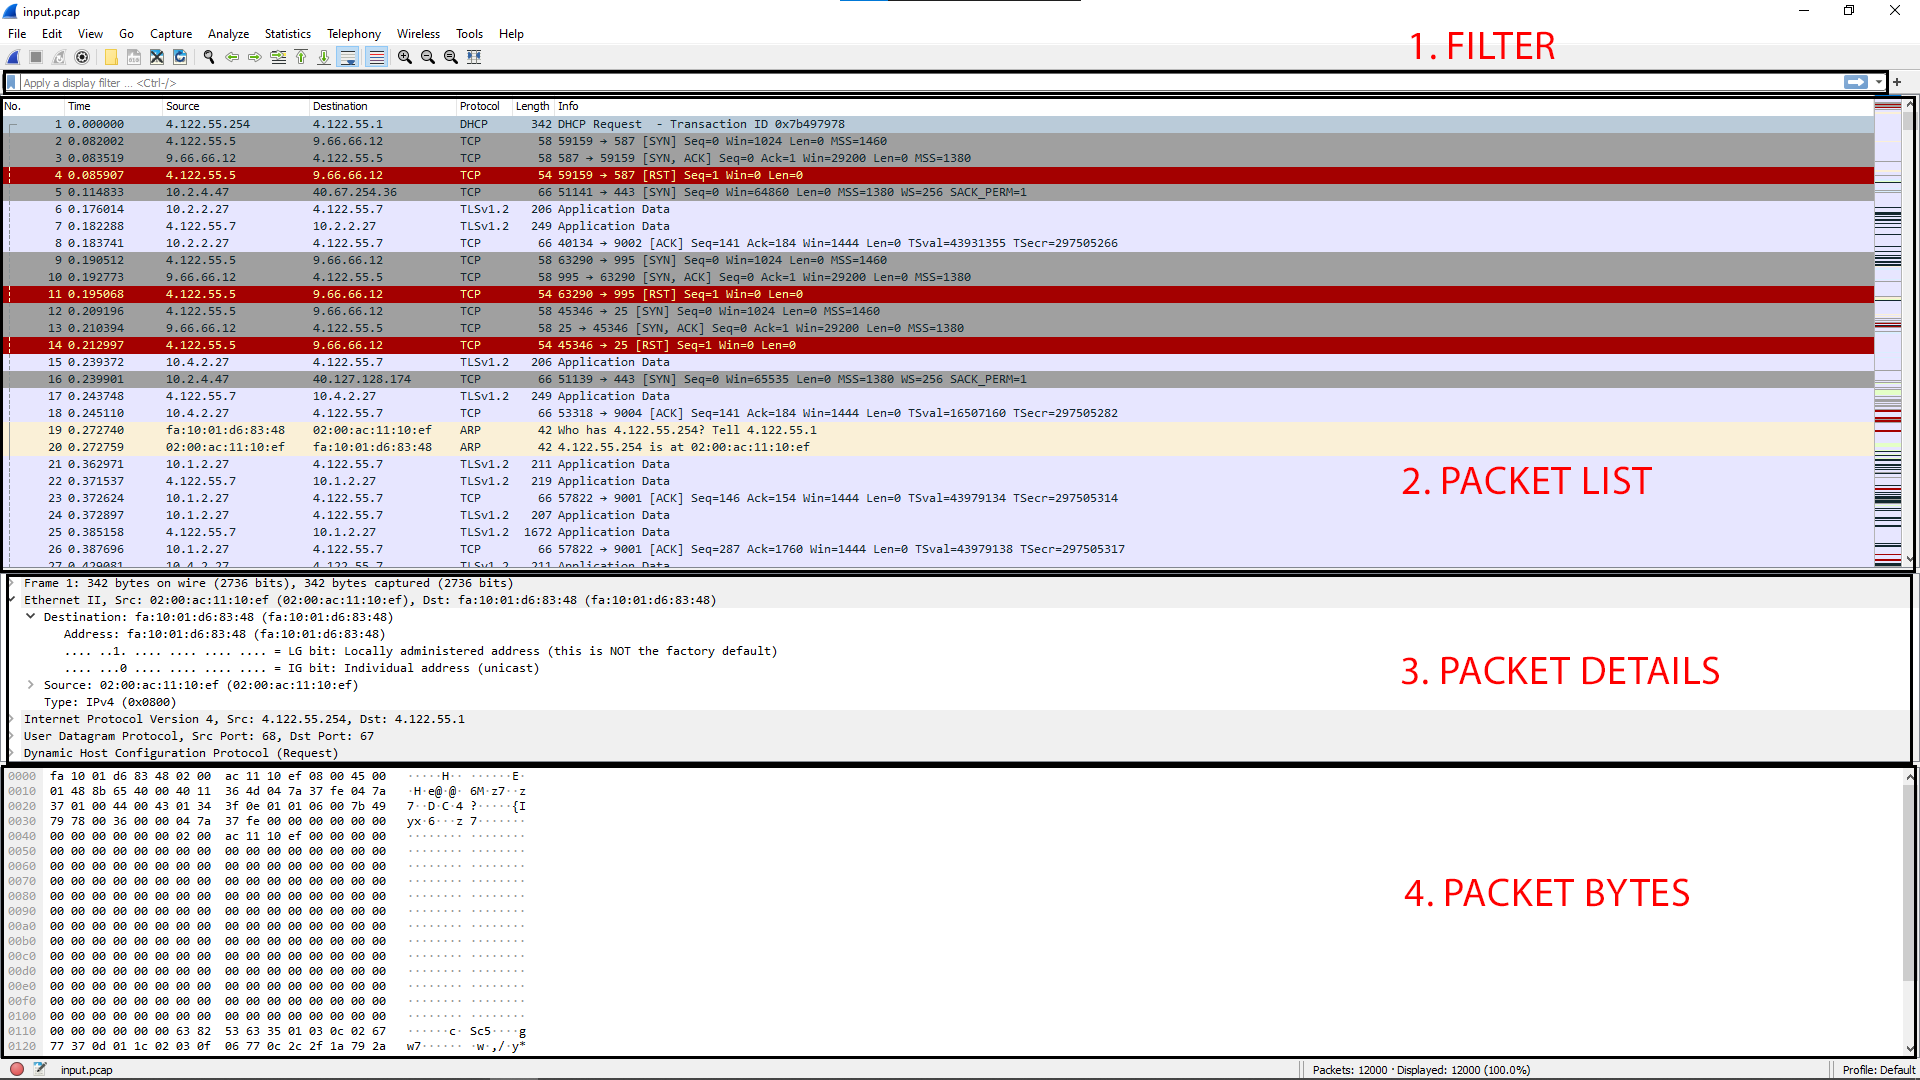
\includegraphics[width=1\textwidth]{images/wireshark_text.png}
  \end{center}
  \caption{The Wireshark GUI interface}
  \label{fig:wireshark}
\end{figure}

\subsection{tcpdump}

Many network administrators often like to use a~command line interface instead of a~GUI because it is often faster and for a~professional clearer to use it this way. It allows for scripting, scheduling jobs, and automatization. One application that offers this and is very feature-rich is tcpdump~\cite{Anintrod85:online}. It comes pre-installed on many Linux distributions and can be used to collect data and analyze them later while being very effective while doing so. 

By dumping the network traffic, tcpdump prints the data of a~given packet on the network interface that is being monitored. We can also use multiple filters to filter only the data that we are interested in. By running the application without any options, it starts to listen to the network on the default interface of a~given machine and dump the packets as they appear on the network. It will, however, require administrator rights in order to access the given interface. It has very low overhead and almost no effect on system resources. To further tune the application to our desired functionality, we can use multiple options and filters to adjust it to our needs\footnote{\url{https://linux.die.net/man/8/tcpdump}}. Tcpdump has many usages, and the options parameters turn specific functionality on or off. There is also the possibility for highly customized filtering. Capturing everything on a~given interface and showing it on the standard output can be done using the \textit{-i} option as shown in the Listing \ref{lst:all}. In order to show just the traffic for a~specific host address, it is possible to specify this address using the \textit{host} option as shown in the Listing \ref{lst:ip}. Filters can be further combined, or the captured packets can be directly saved to the capture file, which is shown in the Listing \ref{lst:file}.

\begin{lstlisting}[language=bash, caption={Capture everything on given interface}, label={lst:all}]
tcpdump -i eth0
\end{lstlisting}

\begin{lstlisting}[language=bash, caption={Filter just the traffic going to or from given address}, label={lst:ip}]
tcpdump host 192.168.1.1
\end{lstlisting}

\begin{lstlisting}[language=bash, caption={Filter the traffic on the port 80, save it to the specified file}, label={lst:file}]
tcpdump port 80 -w capture_file.pcap
\end{lstlisting}

\subsection{tshark}

Tshark is another command line tool that is, like tcpdump, used by many administrators in order to automatize network monitoring and troubleshooting. As its name reveals, it is part of Wireshark that is available on the command line interface~\cite{tshark112:online}. Compared to tcpdump, it provides even more advanced filtering options and scripting capabilities. It supports much more file formats and can read packet captures generated by other tools. It requires more system resources and is generally for more advanced users. Without any options provided, tshark will act much like tcpdump so that it will dump the network data of the default interface to the command line. Tshark is a~free and open-source tool that comes installed with Wireshark and offers advanced filtering options. While many code snippets would be similar to tcpdump, there would also be many differences. Tshark uses different syntax and offers even more customizability and output options. It has support for more protocols and can print out more information about captured packets as well as statistics. For example, it is possible to display the amount of data captured for each packet. This is shown in the Listing \ref{lst:tsharkdata}. Additionally, tshark offers advanced filtering options. These include filtering just the packets where the value of a~field is in a~certain range, as shown in the Listing \ref{lst:tsharkfilter}. And just like tcpdump, tshark can also save the packets to the capture file, which could later be used for analysis, as shown in the Listing \ref{lst:tsharksave}.

\begin{lstlisting}[language=bash, caption={Display amount of data captured per packet}, label={lst:tsharkdata}]
tshark -i eth0 -T fields -e frame.len
\end{lstlisting}

\begin{lstlisting}[language=bash, caption={Filter by the value in a~certain range}, label={lst:tsharkfilter}]
tshark -i eth0 -Y "tcp.window_size >= 8192 && tcp.window_size < 16384"
\end{lstlisting}

\begin{lstlisting}[language=bash, caption={Save capture to pcap file}, label={lst:tsharksave}]
tshark -i eth0 -w capture.pcap
\end{lstlisting}



\section{Challenges of data capture}

While capturing digital data, there are many challenges that we first need to think about in order to account for them while gathering the data. When not thought about deeply, some of these challenges may actually cause more harm than one could imagine. That is why it is very important to make sure we understand them. It is important to understand the principles of network monitoring and the network itself to identify these challenges. We must also think about the challenges from a packet trace manipulation perspective, and understand the implications that the packet trace manipulation brings.

\subsection{New protocols}

As the Internet itself and networks are still evolving, many new protocols are brought to use every month~\cite{Examinin23:online}. While monitoring the network traffic, it is important to account for this fact. Attackers may use these new protocols to develop new types of attacks, which older monitoring software or detection methods might not be able to discover in time or at all. The detection methods implemented in software that would be used to detect the modifications made to a packet capture might be obsolete, and this can serve as a way for attackers to hide the traces. By leveraging the use of newer protocols, attackers may hide the malicious activity in the packet trace files by gaining access to the packet trace and modifying the traffic to hide behind these new unsupported protocols.

This includes newer protocols like QUIC~\cite{RFC9000}, technologies like cloud computing, and IoT devices, which are able to generate massive amounts of network traffic in a~matter of seconds. To meet these new standards, monitoring software should be scalable and able to adapt to changing environments, which further requires ongoing research on this topic. Therefore, it is important to think about the challenges that the new protocols and technologies bring to the world of network monitoring and forensic analysis of network packet captures. Attackers might use this knowledge to alter the packet trace file in such a way that they will inject decoy packets in the form of a large number of packets with huge payloads to hinder the detection process.

One of the protocols that have the potential to change the way we think about network monitoring and packet captures is the \textbf{QUIC} (Quick UDP Internet Connections) protocol. Originally designed by Google, but currently maintained by IETF to standardize its usage, generalized under RFC9000. The main reason for this protocol to exist is to overcome some limitations of TCP/TLS connections. It is also used to improve the experience of web users by reducing web page load times, as it is based on UDP protocol which is connectionless. It uses port 443, and because it is connectionless by the standard, it has no guaranteed delivery of packets. This means that all the necessary functions to ensure data delivery has to be implemented by the QUIC protocol. This protocol, however, brings considerable challenges when it comes to network monitoring. 

\begin{itemize}
    \item \textbf{Encryption} By design, all data that are transferred using QUIC protocol are always encrypted. This means that while packet capture is still without significant problems, further analysis is complicated, impossible, or requires decryption algorithms. It might also mean that some data will never be recovered at all. This can be used to hide malicious acts in packet traces by manipulating the payloads of the packets.
    \item \textbf{Support} QUIC is relatively new, which means it is not supported by many applications and hardware. This opens security holes and could be used by attackers. Many network monitoring solutions work with HTTP and HTTPS traffic transferred over TCP or TCP+TLS protocols and might not yet understand QUIC. Modification detection software might not be ready for these types of attacks.
    \item \textbf{Versions} There are many different versions of QUIC on the internet, making network monitoring difficult. In order to monitor the protocol, we need to know the exact specifications of the given version. If there are many versions, it might not be possible to do it effectively.
\end{itemize}

\subsection{Storing the data for further analysis}

In order to make use of passive monitoring, we need to have reliable storage methods for the network traffic. By saving each packet on the network, we ensure that the traffic can, in fact, be analyzed later and can be used as proof against the criminal act~\cite{ABBASI202119}. It can therefore play a~huge role in forensics and be a~crucial part of the investigation. To store the data, we usually use the PCAP or PCAPNG formats mentioned in this chapter already. 

This can, however, lead to storing huge amounts of data. These also have to be analyzed later, so it is not wise to delete them. Also, having huge files may propose performance problems for monitoring and detection algorithms and applications. In order to store the data, one must think about how much data to expect. This can vary hugely depending on network size, number of devices on the network, expected traffic, and other factors. Storing terabytes of data is not always feasible, and thus it is important to consider storage options. Relational databases and some types of file-based storage options or NAS might not be suitable for real-time capture due to latency. Local file-based storage also can not be easily scalable. Object storage on platforms like Amazon S3\footnote{\url{https://aws.amazon.com/s3/}} or Azure Blob Storage\footnote{\url{https://azure.microsoft.com/en-us/products/storage/blobs}} are scalable and provide fast access to data, but again, might not be useful for real-time capture.

There will also be some "noise" in the captured traffic. Meaning that there will be some data that will not be useful for the analysis, but they are still present in the PCAP(NG) file. These data can then significantly increase the amount of data to be stored and also increase the size of the PCAP(NG) file. It is then much harder to work with terabytes worth of PCAP(NG) files, and the analysis can take exponentially longer.

\subsection{Other limitations}

Because this thesis focuses on offline monitoring and relies on packet captures, there are some more limitations that I myself have encountered while working on this thesis. These consist of the following:
\begin{itemize}
\item \textbf{Incomplete data:} After packet capture is acquired, it does not necessarily need to contain all the sufficient data. The capture could have started too late or ended prematurely. This can have a~high negative impact on modification detection, as we lack the complete image and might miss important information.

\item \textbf{Corrupted data:} We can think of corrupted data as \textit{incomplete} in such a~way that it might never be possible to recover them. Captured data can be corrupted while transferring the file or while manipulating it in any way. Corruption may also occur without direct user interaction, simply by storing the data on a~faulty drive.

\item \textbf{Usage of nonstandard ports:} It is also quite common for many applications and software to use nonstandard ports for communication. According to Internet Assigned Numbers Authority (IANA), there should be standard and nonstandard ports that should or should not be used by any given application\footnote{\url{https://www.iana.org/assignments/service-names-port-numbers/service-names-port-numbers.xhtml}}. However, it does not prohibit any application to use any port it desires, as long as it is open and free to use. This means that we can not rely completely on this list alone.

\item \textbf{Packet loss:} Packet loss is something that is quite common on networks~\cite{4594875}. It might occur even on healthy networks and is part of the internet. SPAN ports can be overloaded and thus not forward any more data. The data-capturing device might also be overloaded. In case of overloading, capturing does not behave in a~predictable way and might therefore lead to packet loss. We must account for that and take it as it is since it is considered normal behavior.

Losing packets is something that can occur on wired networks as well as on wireless ones. However, it is much more common for it to occur on wireless networks because there is much more interference and other crucial factors that allow this.

Many studies attribute the primary source of wireless losses to errors in a~physical medium. However, one study from 2008~\cite{4594875} shows that this might not be the case, as they found that the correlation between multiple closely located receivers was low, with the majority of loss instances only occurring at one of the specific receivers. It also shows that wireless cards might be the culprit. While they operate similarly on the macro level, there are huge differences on the micro level, which consist of data consistency and latency.

\end{itemize}


These limitations show that the captures conducted on the wireless network might show more errors, and the data might be more incomplete, leading to a~lesser quality of packet capture files with fewer data which can lead to false positive conclusions. Understanding these limitations and challenges will help us to prevent making early conclusions based on incomplete and misleading data. Assigning high importance to these factors would be a~great mistake while evaluating packet capture modification.


\section{Understanding network protocols}
\label{chap:protocols}

Network protocols or communication protocols are a~set of rules that allow two or more devices to transmit information over some kind of communication channel. Protocol usually defines rules, syntax, semantics, and synchronization methods for the communication parties~\cite{Espacene23:online}. They play a~critical role in the network monitoring world because their function, as well as rules, content, and usage, determines what kind of data we are expected to see transmitted by them. Therefore, it is important to describe the most important ones in terms of their role in the network and the differences between them. Many protocols are similar. Many share just some basics, and some protocols directly influence others.

By the nature of the TCP/IP model, multiple protocols often cooperate with each other in order to achieve the functionality they offer~\cite{10.5555/2584507}. Protocols in the Application Layer rely on Transport Layer protocols to provide reliable data delivery between applications. Here they use TCP protocol, for example. Application Layer protocols use the IP protocol to router packets between different hosts on the Internet or Link Layer protocols like Ethernet or 802.11. HTTPS is an example of an Application Layer protocol where the usage spans not only across multiple layers but can also work in cooperation with DNS protocol on the Application Layer, which takes care of resolving domain names. Given the TCP/IP model, we can divide the protocols based on their operating layer.


\subsection{Link Layer protocols}

Link layer protocols are at the lowest layer in the Internet protocol suite. It is basically a~group of rules dedicated to the physical connection between the host and the network. It describes Ethernet and other IEEE 802 networks like WiFi~\cite{10.5555/2584507}.

\subsubsection{MAC}
\label{chap:mac}
MAC stands for media access control. It represents a~sublayer of the Link layer whose main task is to control the hardware responsible for communication and information transmission. It is directly responsible for encapsulating the information into frames and transferring them to other network devices. According to IEEE ~\cite{IEEEStd80:online}, the MAC sublayer performs data transfer between stations in support of the LLC sublayer. The MAC frame is then used to describe the packets transferred within the MAC layer, and the main functions of the MAC sublayer are the following:

\begin{itemize}[noitemsep,topsep=0pt]
    \item Frame delimiting and recognition
    \item Addressing of destination stations(individual as well as groups)
    \item Conveyance of source-station addressing information
    \item Transparent data transfer of LLC PDUs
    \item Error correction
    \item Control of access to the physical transmission medium
\end{itemize}

\bigskip
Addressing in the MAC sublayer is done using a~MAC address. a~MAC address is a~link-layer address that is sometimes also called a~LAN address or a~physical address. And because it is managed by IEEE, it is guaranteed that there are no collisions worldwide. That is because it is embedded in the hardware of the networking card itself. MAC address is 6 bytes long and typically expressed in hexadecimal notation.

By design, no two adapters or network cards have the same MAC address. However, the MAC address can still be edited by the end user. Example of MAC address:

\begin{center}
    FF-FF-FF-FF-FF-FF
\end{center}

The Ethernet frame consists of various fields, which are shown in Figure \ref{fig:mac_frame}. Each field has its purpose. While some are optional, like extensions, others are required.

\begin{itemize}[noitemsep,topsep=0pt]
    \item \textbf{Preamble field:} MAC frame starts with Preamble field. This is a~7--octet field used to establish bit synchronization.
    \item \textbf{SFD:} This is a~1--octet field that is always a~sequence 10101011. Always follows the Preamble. MAC frame starts immediately after SFD.
    \item \textbf{Address fields:} Each MAC frame contains Destination and Source address fields in this order. The destination address specifies the addressee or addressees for which the MAC frame is intended. The source address identifies the host from which the frame originated. Each address field is exactly six octets long.
    \item \textbf{Length/type field:} Represented in two octets, the Length/Type field is a~field that takes one of the two meanings, depending on its value. If the value is less than or equal to 1500, it indicates the length of data octets. If this value is greater, it indicates EtherType, the type interpretation of protocol.
    \item \textbf{MAC Client data field:} This field contains a~sequence of data octets.
    \item \textbf{PAD field:} For a~MAC frame, a~minimum frame size is provided. If the length of the MAC Client data field is insufficient, a~PAD field is appended after the MAC Client data field.
    \item \textbf{Frame check sequence field:} 4--octet field that contains CRC (Cyclic Redundancy Check) value. It is generated over the destination address, source address, length, and a~data field. The packet is considered corrupted if the checksum computed by the destination is not the same as in the source checksum.
\end{itemize}


\begin{figure}[h]
\fontsize{7pt}{7pt}\selectfont
\begin{center}
\begin{BVerbatim}
 0                   1                   2                   3                   4              
 0 1 2 3 4 5 6 7 8 9 0 1 2 3 4 5 6 7 8 9 0 1 2 3 4 5 6 7 8 9 0 1 2 3 4 5 6 7 8 9 0 1 2 3 4 5 6 7
+-+-+-+-+-+-+-+-+-+-+-+-+-+-+-+-+-+-+-+-+-+-+-+-+-+-+-+-+-+-+-+-+-+-+-+-+-+-+-+-+-+-+-+-+-+-+-+-+
|                                      Destination Address                                      |
+-+-+-+-+-+-+-+-+-+-+-+-+-+-+-+-+-+-+-+-+-+-+-+-+-+-+-+-+-+-+-+-+-+-+-+-+-+-+-+-+-+-+-+-+-+-+-+-+
|                                         Source Address                                        |
+-+-+-+-+-+-+-+-+-+-+-+-+-+-+-+-+-+-+-+-+-+-+-+-+-+-+-+-+-+-+-+-+-+-+-+-+-+-+-+-+-+-+-+-+-+-+-+-+
|           EtherType           |                                                               |
+-+-+-+-+-+-+-+-+-+-+-+-+-+-+-+-+                                                               +
|                                                                                               |
+                                            Payload                                            +
|                                                                                               |
+-+-+-+-+-+-+-+-+-+-+-+-+-+-+-+-+-+-+-+-+-+-+-+-+-+-+-+-+-+-+-+-+-+-+-+-+-+-+-+-+-+-+-+-+-+-+-+-+
\end{BVerbatim}
  \end{center}
  \caption{Ethernet frame packet format~\cite{9844436}}
  \label{fig:mac_frame}
\end{figure}

By using the MAC sublayer, two devices are able to communicate on LAN and exchange information. This, however, will not work without ARP protocol and IP addresses.

\subsubsection{ARP}
\label{sec:arp}

ARP stands for Address Resolution Protocol~\cite{10.5555/2584507}. It acts as some kind of translator between the Link layer and the Internet layer. ARP, therefore, is used to map the IP address to its corresponding MAC address. Given that MAC addresses are unique, ARP allows seamless communication between devices on the network.

\medskip

Let us consider a~device that wants to send information data to another device on the same network. Firstly, it checks its ARP cache. ARP cache contains a~map of all IP addresses to MAC addresses that the device has previously discovered. If the IP of the device it wants to send data to is in the ARP cache, the device can use the corresponding MAC address to send data to the destination. However, this cache only lasts a~limited amount of time in order for the changes on the network to be actualized.

If the destination IP address is not in the ARP cache, it is considered an ARP miss. Sending device has to somehow get the MAC address of the destination device from the network. Therefore, the sending device broadcasts an ARP request message to all devices on the given network, asking for a~MAC address of the device with the given destination IP. This request contains information about the sending device as well as the IP of the destination machine. When the destination device receives the ARP request message, it then checks its IP address and then checks if it matches the IP address that came in the ARP request message. If it does not, it discards this packet as if nothing happened.

If the device matches the IP address in the ARP request, it sends an ARP response message to the sender's MAC address. This message contains the IP and MAC address of the device that the ARP request message required.

ARP packet structure is described in RFC 826~\cite{RFC0826}. It specifies the ARP protocol and describes how ARP packets are used to resolve network-layer addresses to link-layer addresses. Notice the protocol address, which refers to the address of the network protocol being used, typically the IP address.

\begin{itemize}[noitemsep,topsep=0pt]
    \item \textbf{Hardware Type:} A~16-bit field that specifies the type of hardware address being used.
    \item \textbf{Protocol Type}: A~16-bit field specifying the type of protocol address used.
    \item \textbf{Hw Addr Len}: An 8-bit field that specifies the length of each hardware address in bytes.
    \item \textbf{Prot Addr Len}: An 8-bit field that specifies the length of each protocol address in bytes.
    \item \textbf{Opcode}: A~16-bit field that indicates whether the ARP packet is a~request or a~response.
    \item \textbf{Sender MAC Address}: The MAC address of the device sending the ARP packet.
    \item \textbf{Sender Protocol Address}: The IP address of the device sending the ARP packet.
    \item \textbf{Target MAC Address}: The MAC address of the device to which the ARP packet is being sent.
    \item \textbf{Target Protocol Address}: The IP address of the device that the ARP packet is being sent to.
\end{itemize}

\medskip 

ARP is essential for the network because it is able to translate addresses between different layers of the TCP/IP model, inherently making it one of the most important protocols of the link layer.



\subsection{Internet Layer protocols}

The network layer is the second layer in the TCP/IP model~\cite{10.5555/2584507}. It is responsible for routing and forwarding data between different networks. It also directly provides addressing, which allows different devices on different networks to communicate with each other using the IP protocol. The network protocol itself is also responsible for the flow of data packets to ensure they reach the target destination in the correct order without any error. The network layer enables communication between devices that are not directly connected to each other. It is responsible for routing, forwarding, and error correction for the transferred packets of data.

\subsubsection{The Internet Protocol}
\label{chap:ip}
The Internet Protocol is the primary protocol used for communication between devices on the Internet. IP provides a~standard for the data packet transmission from one device to another device over a~network. It is responsible for routing packets between devices by assigning unique IP addresses and determining the best path for the data to travel in order to reach the destination. Some of the algorithms used for pathfinding include Shortest Path First(SPF), Dijkstra's algorithm, or the Bellman-Ford algorithm.

IP is also connectionless. This means that it does not in any way establish a~dedicated connection between devices before transmitting. Instead, it takes care of breaking data down into smaller chunks called packets. Afterward, it sends these packets individually over the network. Each packet then contains the destination IP address and other necessary information needed for routing across the different networks.

 Currently, there are two versions of IP: IPv4 and IPv6. IPv4 is older and more widely used, while IPv6 is becoming increasingly popular because it allows for a~vastly larger number of IP addresses in the network.

 The main differences between these versions are the following:

 \begin{itemize}[noitemsep,topsep=0pt]
     \item \textbf{Address space}: IPv6 allows for much more unique IP addresses than the IPv4.
     \item \textbf{Security}: IPv6 has in-built security features like IPsec or traffic encryption
     \item \textbf{Autoconfiguration}: IPv6 provides automatic address configuration. This eliminates the need for DHCP or manual configuration of IP addresses.
 \end{itemize}

 \paragraph{IPv4} uses 32 bits to store the address. This limits the total number of unique addresses to around 4.3 billion. It consists of two main parts: header and data. The IPv4 header has a variable size with a minimum of 160 bits and a maximum of 480 bits for its structure. This may contain several fields that are used to help deliver packets to their destination, including Version, Type of Service, and many more. The optional parameter \texttt{options} can increase the header size exponentially, based on the options provided in the given packet.
 
 The IPv4 address then looks like this:

 \begin{center}
    192.168.1.1
\end{center}

The format~\cite{RFC0791} of the Internet Header shown in Figure \ref{fig:ip_header} represents the IPv4 protocol's header format and its fields.

\begin{itemize}[noitemsep,topsep=0pt]
    \item \textbf{Version}: A~4-bit field that specifies the version of the Internet Protocol (IP) being used.
    \item \textbf{Header Length}: A~4-bit field specifying the IP header's length in 32-bit words.
    \item \textbf{Type of Service (TOS)}: An 8-bit field that provides information about the priority and nature of the data being carried by the IP packet.
    \item \textbf{Total Length}: A~16-bit field that specifies the total length of the IP packet, including the header and data.
    \item \textbf{Identification}: A~16-bit field that provides a~unique identifier for the IP packet, which can be used to fragment and reassemble the packet.
    \item \textbf{Flags}: A~3-bit field that provides control information for packet fragmentation and reassembly.
    \item \textbf{Fragment Offset}: A~13-bit field specifying the offset of the data in the current fragment relative to the start of the original packet.
    \item \textbf{Time to Live (TTL)}: An 8-bit field that specifies the maximum number of hops that the IP packet can take before being discarded.
    \item \textbf{Protocol}: An 8-bit field identifying the protocol used in the data portion of the IP packet.
    \item \textbf{Header Checksum}: A~16-bit field that provides error detection for the IP header.
    \item \textbf{Source Address}: A~32-bit field that specifies the IP address of the sender of the packet.
    \item \textbf{Destination Address}: A~32-bit field that specifies the IP address of the intended recipient of the packet.
    \item \textbf{Options}: An optional variable-length field that can be used to include additional information in the IP header.
    \item \textbf{Padding}: A~variable-length field that can be used to ensure that the total length of the IP header is a~multiple of 32 bits.
\end{itemize}

\begin{figure}[h]
\fontsize{10pt}{10pt}\selectfont
\begin{center}
\begin{BVerbatim}
 0                   1                   2                   3  
 0 1 2 3 4 5 6 7 8 9 0 1 2 3 4 5 6 7 8 9 0 1 2 3 4 5 6 7 8 9 0 1
+-+-+-+-+-+-+-+-+-+-+-+-+-+-+-+-+-+-+-+-+-+-+-+-+-+-+-+-+-+-+-+-+
|Version|  IHL  |Type of Service|          Total Length         |
+-+-+-+-+-+-+-+-+-+-+-+-+-+-+-+-+-+-+-+-+-+-+-+-+-+-+-+-+-+-+-+-+
|         Identification        |Flags|     Fragment Offset     |
+-+-+-+-+-+-+-+-+-+-+-+-+-+-+-+-+-+-+-+-+-+-+-+-+-+-+-+-+-+-+-+-+
|  Time to Live |    Protocol   |        Header Checksum        |
+-+-+-+-+-+-+-+-+-+-+-+-+-+-+-+-+-+-+-+-+-+-+-+-+-+-+-+-+-+-+-+-+
|                         Source Address                        |
+-+-+-+-+-+-+-+-+-+-+-+-+-+-+-+-+-+-+-+-+-+-+-+-+-+-+-+-+-+-+-+-+
|                      Destination Address                      |
+-+-+-+-+-+-+-+-+-+-+-+-+-+-+-+-+-+-+-+-+-+-+-+-+-+-+-+-+-+-+-+-+
|                    Options                    |    Padding    |
+-+-+-+-+-+-+-+-+-+-+-+-+-+-+-+-+-+-+-+-+-+-+-+-+-+-+-+-+-+-+-+-+
\end{BVerbatim}
\end{center}
  \caption{IPv4 Header~\cite{RFC0791}}
  \label{fig:ip_header}
\end{figure}

 \paragraph{IPv6}, on the other hand, represents a~newer and much more advanced version of the Internet Protocol. It uses 128-bit long addresses, which allows for an exponentially larger amount of unique addresses. Similarly, IPv6 also consists of two parts, header and data. The header is now 320 bits long, which is the consequence of the much longer addresses.

 The IPv6 address then looks like this:

 \begin{center}
    1111:2222:3333:4444:CCCC:DDDD:EEEE:FFFF
\end{center}

The format~\cite{RFC2460} of the Internet Header shown in Figure \ref{fig:ipv6_header} represents the IPv6 protocol's header format and its fields.

\begin{itemize}[noitemsep,topsep=0pt]
    \item \textbf{Version}: A~4-bit field that specifies the version of the Internet Protocol (IP) being used.
    \item \textbf{Traffic Class}: An 8-bit field that provides QoS (Quality of Service) and ECN (Explicit Congestion Notification) information.
    \item \textbf{Flow Label}: A~20-bit field that identifies a~flow of packets that requires special handling.
    \item \textbf{Payload Length}: A~16-bit field specifying the payload length (data) in the packet, excluding the header.
    \item \textbf{Next Header}: An 8-bit field that identifies the protocol used in the data portion of the packet.
    \item \textbf{Hop Limit}: An 8-bit field specifying the maximum number of hops the packet can take before being discarded.
    \item \textbf{Source Address}: A~128-bit field specifying the IP address of the packet's sender.
    \item \textbf{Destination Address}: A~128-bit field that specifies the IP address of the intended recipient of the packet.
\end{itemize}

\begin{figure}[h]
\fontsize{10pt}{10pt}\selectfont
\begin{center}
\begin{BVerbatim}
 0                   1                   2                   3  
 0 1 2 3 4 5 6 7 8 9 0 1 2 3 4 5 6 7 8 9 0 1 2 3 4 5 6 7 8 9 0 1
+-+-+-+-+-+-+-+-+-+-+-+-+-+-+-+-+-+-+-+-+-+-+-+-+-+-+-+-+-+-+-+-+
|Version| Traffic Class |               Flow Label              |
+-+-+-+-+-+-+-+-+-+-+-+-+-+-+-+-+-+-+-+-+-+-+-+-+-+-+-+-+-+-+-+-+
|         Payload Length        |  Next Header  |   Hop Limit   |
+-+-+-+-+-+-+-+-+-+-+-+-+-+-+-+-+-+-+-+-+-+-+-+-+-+-+-+-+-+-+-+-+
|                                                               |
+                                                               +
|                                                               |
+                         Source Address                        +
|                                                               |
+                                                               +
|                                                               |
+-+-+-+-+-+-+-+-+-+-+-+-+-+-+-+-+-+-+-+-+-+-+-+-+-+-+-+-+-+-+-+-+
|                                                               |
+                                                               +
|                                                               |
+                       Destination Address                     +
|                                                               |
+                                                               +
|                                                               |
+-+-+-+-+-+-+-+-+-+-+-+-+-+-+-+-+-+-+-+-+-+-+-+-+-+-+-+-+-+-+-+-+
\end{BVerbatim}
\end{center}
  \caption{IPv6 Header~\cite{RFC2460}}
  \label{fig:ipv6_header}
\end{figure}


\bigskip

Given that both versions are currently used simultaneously, there must be a~way of translating between IPv4 address space and IPv6 address space. The problem is that while IPv6 is backwards compatible with IPv4 using tunneling, the IPv4-only capable systems are incapable of handling IPv6 datagrams. This then has to be resolved, for example, by using a~dual-stack approach where a~device with IPv6 also implements IPv4~\cite{10.5555/2584507}.

\subsubsection{ICMP}

ICMP stands for Internet Control Message Protocol~\cite{RFC0792}. It is one of the most important protocols, as its main function is to send error messages and operational information about network conditions. It is, therefore, an integral part of the Internet Protocol suite and is used by network devices to communicate with each other.

ICMP works by sending messages that contain information about the network and its status. These messages are sent by routers or other network devices to inform that, for example, the desired destination network is not reachable. ICMP is often considered part of IP, but architecturally it lies just above the IP. This is because ICMP messages are carried inside IP datagrams. One of the well-known programs that utilize ICMP and send them is the ping program, used to test the response time of the destination device.

The structure of the ICMPv4 packet is shown in Figure \ref{fig:icmp}

\begin{figure}[h]
\fontsize{10pt}{10pt}\selectfont
\begin{center}
\begin{BVerbatim}
 0                   1                   2                   3  
 0 1 2 3 4 5 6 7 8 9 0 1 2 3 4 5 6 7 8 9 0 1 2 3 4 5 6 7 8 9 0 1
+-+-+-+-+-+-+-+-+-+-+-+-+-+-+-+-+-+-+-+-+-+-+-+-+-+-+-+-+-+-+-+-+
|      Type     |      Code     |            Checksum           |
+-+-+-+-+-+-+-+-+-+-+-+-+-+-+-+-+-+-+-+-+-+-+-+-+-+-+-+-+-+-+-+-+
|                                                               |
+                          Message Body                         +
|                                                               |
+-+-+-+-+-+-+-+-+-+-+-+-+-+-+-+-+-+-+-+-+-+-+-+-+-+-+-+-+-+-+-+-+
\end{BVerbatim}
\end{center}
  \caption{ICMPv4 general format~\cite{RFC0792}}
  \label{fig:icmp}
\end{figure}

\begin{itemize}[noitemsep,topsep=0pt]
    \item \textbf{Type}: Specifies the type of message, such as Echo Request or Destination Unreachable.
    \item \textbf{Code}: Provides additional information about the message type, such as a~specific error condition.
    \item \textbf{Checksum}: Provides error-checking for the ICMPv4 message.
    \item \textbf{Identifier}: A~16-bit identifier that can be used to match requests and replies.
    \item \textbf{Sequence Number}: A~16-bit number that can be used to match requests and replies.
    \item \textbf{Message Body}: Contains additional information about the message, such as an error message or the payload of an Echo Request/Reply message.
\end{itemize}

There are many different messages that ICMP can send. Some of the common types are the following~\cite{10.5555/2584507}:

\begin{itemize}[noitemsep,topsep=0pt]
    \item \textbf{Echo Request and Echo Reply}: These messages are typically used to test the reachability of a~network device or measure the round-trip time for packets. They are often used by the ping program.
    \item \textbf{Destination Unreachable}: This message is sent by a~router to inform the sender that the route to the destination network can not be found.
    \item \textbf{Time Exceeded}: Is used to inform the sender that the packet was discarded because it exceeded the maximum time to live value(TTL).
\end{itemize}

\subsection{Transport Layer protocols}

The transport layer is a~layer in the TCP/IP networking model that manages the communication between two network endpoints by providing reliable, end-to-end data transport services. The main functions of this layer are data segmenting into smaller packets and their reassembly, providing reliable data delivery through error detection and correction, flow control, multiplexing, and demultiplexing, and establishing a~connection between devices.

\subsubsection{UDP}

UDP stands for User Datagram Protocol, and it represents another protocol from the Internet Protocol suite. This protocol is used for transmitting data over networks. UDP is, however, a~connectionless protocol. This means that it does not establish a~dedicated connection between the two endpoints transmitting data. This can lead to various problems, but it simplifies the protocol and makes it lightweight while still being fast and good enough for some applications like video conferencing.

UDP simply packages data into diagrams and sends them over to another network. Each datagram is then independent and can be delivered sooner or later than the previous. UDP does not guarantee data delivery or packet order. This might seem like a~significant disadvantage, but UDP also offers some advantages in certain situations. These represent the speed for transferring some amount of data because it does not require any overhead. This can be useful for real-time audio or video applications.

Note that the UDP header is relatively simple, consisting only of four fields~\cite{RFC0768}, as shown in Figure \ref{fig:udp}.

\begin{itemize}[noitemsep,topsep=0pt]
    \item \textbf{Source Port}: A~16-bit field that specifies the source port number.
    \item \textbf{Destination Port}: A~16-bit field that specifies the destination port number.
    \item \textbf{Length}: A~16-bit field that specifies the length of the UDP packet in bytes, including the header and data.
    \item \textbf{Checksum}: A~16-bit field that provides error-checking for the UDP packet.
    \item \textbf{Data}: The payload of the UDP packet, can be up to 65,535 bytes in length.
\end{itemize}

\begin{figure}[h]
\fontsize{10pt}{10pt}\selectfont
\begin{center}
\begin{BVerbatim}
 0                   1                   2                   3  
 0 1 2 3 4 5 6 7 8 9 0 1 2 3 4 5 6 7 8 9 0 1 2 3 4 5 6 7 8 9 0 1
+-+-+-+-+-+-+-+-+-+-+-+-+-+-+-+-+-+-+-+-+-+-+-+-+-+-+-+-+-+-+-+-+
|          Source Port          |        Destination Port       |
+-+-+-+-+-+-+-+-+-+-+-+-+-+-+-+-+-+-+-+-+-+-+-+-+-+-+-+-+-+-+-+-+
|             Length            |            Checksum           |
+-+-+-+-+-+-+-+-+-+-+-+-+-+-+-+-+-+-+-+-+-+-+-+-+-+-+-+-+-+-+-+-+
\end{BVerbatim}
\end{center}
  \caption{UDP header~\cite{RFC0768}}
  \label{fig:udp}
\end{figure}

\subsubsection{TCP}
\label{chap:tcp}
Unlike UDP, TCP(Transmission Control Protocol)~\cite{RFC0793} establishes a~direct connection between two devices that want to transmit data over the network. TCP then provides reliable, connection-oriented, ordered data delivery between applications running on these connected devices. TCP inherently ensures that the packets are ordered correctly and that the transmission of all packets is reliable and without errors.

Firstly, a~connection between two devices is established using a~three-way handshake. During this handshake, two communicating devices exchange special packets called SYN and ACK to establish the connection. Once it is established, actual data can be transmitted in both directions. Including features such as flow control and congestion control to manage the flow of data over the network, TCP ensures the quality and reliability of the transmission. Flow control directly ensures that the sender does not send too much data too quickly, while congestion control prevents the network from becoming overloaded.

TCP header, when compared to UDP, is much more complex. Notable are the several additional fields like a~sequence number, acknowledgment number, and others.

\begin{itemize}[noitemsep,topsep=0pt]
    \item \textbf{Source Port}: a~16-bit field that provides the source port number.
    \item \textbf{Destination Port}: a~16-bit field specifying the destination port number.
    \item \textbf{Sequence Number}: a~32-bit field specifying the sequence number of the first data byte in the TCP segment.
    \item \textbf{Acknowledgment Number}: a~32-bit field that specifies the sequence number of the next expected data byte in the TCP segment.
    \item \textbf{Data Offset}: a~4-bit field specifying the length of the TCP header in 32-bit words.
    \item \textbf{Reserved}: a~3-bit field reserved for future use.
    \item \textbf{NS}: a~1-bit flag that is used for ECN (Explicit Congestion Notification).
    \item \textbf{Control Flags}: a~9-bit field containing various control flags such as SYN, ACK, RST, etc.
    \item \textbf{Window Size}: a~16-bit field that specifies the size of the receive window.
    \item \textbf{Checksum}: a~16-bit field that provides error-checking for the TCP segment.
    \item \textbf{Urgent Pointer}: a~16-bit field that communicates the offset from the current sequence number of the last urgent data byte.
    \item \textbf{Options}: An optional field that contains TCP options such as Maximum Segment Size, SACK, etc.
\end{itemize}

\begin{figure}[h]
\fontsize{10pt}{10pt}\selectfont
\begin{center}
\begin{BVerbatim}
    0                   1                   2                   3
    0 1 2 3 4 5 6 7 8 9 0 1 2 3 4 5 6 7 8 9 0 1 2 3 4 5 6 7 8 9 0 1
   +-+-+-+-+-+-+-+-+-+-+-+-+-+-+-+-+-+-+-+-+-+-+-+-+-+-+-+-+-+-+-+-+
   |          Source Port          |       Destination Port        |
   +-+-+-+-+-+-+-+-+-+-+-+-+-+-+-+-+-+-+-+-+-+-+-+-+-+-+-+-+-+-+-+-+
   |                        Sequence Number                        |
   +-+-+-+-+-+-+-+-+-+-+-+-+-+-+-+-+-+-+-+-+-+-+-+-+-+-+-+-+-+-+-+-+
   |                    Acknowledgment Number                      |
   +-+-+-+-+-+-+-+-+-+-+-+-+-+-+-+-+-+-+-+-+-+-+-+-+-+-+-+-+-+-+-+-+
   |  Data |       |C|E|U|A|P|R|S|F|                               |
   | Offset| Rsrvd |W|C|R|C|S|S|Y|I|            Window             |
   |       |       |R|E|G|K|H|T|N|N|                               |
   +-+-+-+-+-+-+-+-+-+-+-+-+-+-+-+-+-+-+-+-+-+-+-+-+-+-+-+-+-+-+-+-+
   |           Checksum            |         Urgent Pointer        |
   +-+-+-+-+-+-+-+-+-+-+-+-+-+-+-+-+-+-+-+-+-+-+-+-+-+-+-+-+-+-+-+-+
   |                           [Options]                           |
   +-+-+-+-+-+-+-+-+-+-+-+-+-+-+-+-+-+-+-+-+-+-+-+-+-+-+-+-+-+-+-+-+
   |                                                               :
   :                             Data                              :
   :                                                               |
   +-+-+-+-+-+-+-+-+-+-+-+-+-+-+-+-+-+-+-+-+-+-+-+-+-+-+-+-+-+-+-+-+
\end{BVerbatim}
\end{center}
  \caption{TCP header~\cite{RFC0793}}
  \label{fig:tcp}
\end{figure}

TCP is one of the most widely used protocols for transmitting data over networks, and it is essential for the functioning of the Internet as we know it today~\cite{10.5555/2584507}. At the beginning of the Internet, TCP played a crucial role in enabling reliable communication between different computer systems. Its importance cannot be overstated, as it laid the foundation for the global connectivity and communication we experience today.

\subsubsection{QUIC}

The QUIC(Quick UDP Internet Connections)~\cite{RFC9000} protocol is a~transport protocol that was developed by Google in 2012. It aims to improve the speed and reliability of internet connections. QUIC was designed to work on top of the UDP instead of TCP because UDP is generally faster and has less overhead. QUIC, however, has to implement the necessary functions in order to be reliable. QUIC also tries to improve its performance overall. The techniques it uses are:

\begin{itemize}
    \item \textbf{Multiplexing}: QUIC allows multiple streams of data to be sent over a~single connection.
    \item \textbf{Encryption}: QUIC encrypts all data it transmits over the network, making it more secure.
    \item \textbf{Congestion control}: QUIC uses congestion control algorithms to avoid network congestion.
\end{itemize}

QUIC also implements \textbf{connection migration}. That means it is able to migrate a~connection from one IP to another. This proves to be significantly important in mobile devices, which tend to switch between cellular and WiFi networks. This protocol also comes with features like \textbf{0-RTT} or 0 Round Trip Time, which allows hosts to send data even before the connection is fully established, further reducing overhead and latency.

\begin{itemize}[noitemsep,topsep=0pt]
    \item \textbf{Header Form (1 bit):} Indicates whether the header is a~long header (0) or a~short header (1).
    \item \textbf{Fixed Bit (1 bit):} Always set to 1 to indicate that the packet is a~QUIC packet.
    \item \textbf{Version (32 bits):} The version of the QUIC protocol being used.
    \item \textbf{Destination Connection ID Length (8 bits):} The length of the destination connection ID.
    \item \textbf{Source Connection ID Length (8 bits):} The length of the source connection ID.
    \item \textbf{Packet Number Length (2 bits):} The length of the packet number in bytes.
    \item \textbf{Reserved Bits (2 bits):} Reserved for future use and set to 0.
    \item \textbf{Packet Number (variable length):} The packet number for this packet.
    \item \textbf{Destination Connection ID (variable length):} The ID of the destination connection.
    \item \textbf{Source Connection ID (variable length):} The ID of the source connection.
    \item \textbf{Payload (variable length):} The payload data of the packet.
\end{itemize}

\medskip

The QUIC protocol changes a~lot about network monitoring because the traffic is now encrypted, there are multiple versions that need to be addressed specifically, and also, the connection migration might bring potential issues with false positives.

\subsection{Application Layer protocols}

The application layer is the topmost layer in the TCP/IP reference model~\cite{10.5555/2584507}. It is responsible for managing the communication services and protocols that allow applications to access the network while exchanging data with other applications. Therefore, it acts as an interface between user application data and the underlying network protocols.

The application layer includes a~wide range of services and protocols spanning from web browsers to email clients or instant messaging applications. Some more examples of application layer protocols are SMTP, used to send emails, FTP for file transfers, or Telnet.

I will now cover the most important services and protocols from the application layer that are essential for this thesis.

\subsubsection{HTTP and HTTPS}

\textbf{HTTP(Hypertext Transfer Protocol)} is a~protocol responsible for handling communication between web servers and web browsers. It is the fundamental part of data communication on the World Wide Web and defines the syntax and semantics of messages exchanged between web servers and clients. HTTP was defined in RFC 1945 and RFC 2616 respectively. It is implemented in two programs: client and server. These programs then talk to each other by exchanging HTTP messages.

\medskip

When a~user requests a~web page by URL(Uniform Resource Locator), the browser sends HTTP request messages for objects in the page to the web server. The server then receives the messages and responds with HTTP response messages containing the requested objects.

HTTP uses TCP as the underlying protocol for data transfer. This means that the transfer is reliable and ordered. Therefore, the client must first establish a~connection with the server by initiating a~TCP connection. The client and server then use sockets to communicate with each other.

HTTP request message typically consists of a~request line, header lines, and message body, while the response message includes a~status line instead of a~request line.

The status line indicates whether the request was successful and provides a~status code. Some of the most common status codes are 200(OK), 404(Not Found), or 500(Internal Server Error).

In itself, HTTP is a~stateless protocol, meaning each request message is independent of any previous one. To overcome this, web browsers store cookies sent over with every request to the server. This small file then identifies specific users and devices.

\medskip

\textbf{HTTPS(Hypertext Transfer Protocol Secure)}~\cite{10.5555/2584507} came shortly after HTTP. It represents a~secure version of HTTP. The difference is HTTPS uses SSL(Secure Socket Layer) or TLS(Transport Layer Security) encryption to create a~secure connection between a~web browser and a~server. This then ensures that any data transmitted between these communicating parties are encrypted. In itself, HTTPS works simply as HTTP. It uses TLS for the transmission rather than HTTP, which uses TCP~\cite{RFC2818}. In contrast, HTTP uses no encryption and sends data in plaintext.

HTTPS is, therefore, much more secure and slowly becoming standard for all websites on the internet. It is crucial for Internet banking applications or e-shops that use private banking data. This also significantly impacts network monitoring, as monitoring encrypted traffic brings many challenges.

\subsubsection{DHCP}

DHCP(Dynamic Host Configuration Protocol)~\cite{RFC2131} represents a~client/server protocol that automatically provides a~host with an IP address and other configuration information, such as the subnet mask or default gateway. DHCP allows hosts to obtain this network information from DHCP servers.

When a~device first connects to a~network, it sends a~request to the DHCP server for an IP address to be assigned. The device knows about the DHCP server because upon connecting to the network, it broadcasts a~DHCPDISCOVER message to discover available DHCP servers. This broadcast message is sent to a~destination IP address 255.255.255.255. DHCP servers receive the message and respond with a~DHCPOFFER message, which includes an available IP address and other network information.

The device then selects an available IP address and confirms it by sending a~DHCP request message for it to be assigned. Afterward, the server sends DHCPACK as an acknowledgment that the IP was assigned to the device, and the device can now communicate with other devices on the network.

DHCP is, therefore, a~mechanism that allows devices to simplify configuration on the network and assign unique IP addresses to that given network.

\subsubsection{DNS}
\label{sec:dns}
In order to identify hosts on the network, we use IP addresses. However, remembering these can be a~tremendous task. Just like telephone directories, the internet uses its own directory service called DNS(Domain Name System). It is a~system that translates domain names such as www.example.com into IP addresses. Computers can not understand domain names directly, so the domain names must be translated using a~DNS server. a~DNS server is a~specific type of server that handles these types of requests.

When a~user enters a~domain name in a~web browser, the browser sends a~DNS query to a~DNS server to resolve the domain name into an IP address. The DNS server looks up the domain name in its database. If the name is found, it takes the associated IP address and returns it to the server. If it is not found, it forwards the query to another server. Once the IP address is received, the browser initiates a~TCP connection to the HTTP server process located at port 80.

The DNS system is hierarchical, where the topmost DNS servers are called root DNS servers. These contain information about top-level domain names such as .com, .org, or others. Below are authoritative DNS servers. These hold specific information about given domain names.

The DNS server and its client communicate using specific types of messages. These include query messages, response messages, or others~\cite{10.5555/2584507}.

\textbf{Query message} contains information about the transaction, flags, question, answer counts, and most importantly, the question section.

The question section contains the following fields:

\begin{itemize}[noitemsep,topsep=0pt]
    \item \textbf{QNAME}: The domain name being requested. This can be, for example, www.example.com
    \item \textbf{QTYPE}: The query type or the type of query being made, such as A(IPv4 address), AAAA(IPv6 address), MX(Mail Exchange), and others.
    \item \textbf{QCLASS}: The class of the query, for example IN(Internet)
\end{itemize}

\textbf{Query answer} is then very similar, with an answer section instead of a~question section. Its answer section then looks like this:

\begin{itemize}[noitemsep,topsep=0pt]
    \item \textbf{NAME}: The domain name that was queried.
    \item \textbf{TYPE}: The type of record being returned.
    \item \textbf{CLASS}: The class of record being returned.
    \item \textbf{TTL}: The time to live for the record, in seconds.
    \item \textbf{RDLENGHT}: The length of the RDATA field in bytes.
    \item \textbf{RDATA}: The actual data containing the information associated with the domain name.
\end{itemize}

\subsubsection{TLS/SSL}

TLS(Transport Layer Security) and SSL(Secure Sockets Layer) represent protocols that provide a~secure communication channel over the Internet~\cite{SSLTLSin60:online}. TLS is the successor to SSL, and the terms are sometimes used interchangeably. TLS/SSL is nowadays used in many modern e-applications, like emails or instant messaging, in order to provide security and privacy. Although TLS is not a~clear application layer protocol, as it operates between the transport layer and the application layer and thus can not be considered as one or the other, it is still a~significant protocol that needs to be addressed.

TLS is considered to be more secure than SSL because TLS uses stronger cryptographic algorithms and key sizes. It has better defenses against known attacks. TLS/SSL works by encrypting data exchanged between two parties and verifying their identity of them. This is done using a~combination of public key and symmetric key cryptography. It, therefore, uses both asymmetric and symmetric cryptography, asymmetric to establish a~secure connection and symmetric to exchange data within this connection. When a~TLS/SSL connection is established, the client and server make sure they have the same TLS/SSL protocol version available. Different versions might not be compatible, so both parties must have the same protocol version installed. Afterward, the client verifies the server's identity using a~digital certificate. This verification is done using The Handshake protocol. This protocol introduces a~series of sequenced messages that inherently negotiate the security parameters of the data transfer. These include the aforementioned version number, session identification, proposed cipher, and more.

After the handshake, communicating parties begin to communicate and exchange data within the secured connection. Nowadays, the most common usages are in HTTPS or aforementioned email or instant messaging applications.



\newpage
\chapter{Modification of captured network data}
\label{chap:modif}

The ability to capture and analyze network traffic is a~crucial component in network forensics to detect and prevent cyberattacks. However, the captured data can often be more complex to understand and interpret without proper knowledge and tools that make it easier. Attackers can even manipulate, modify or obfuscate the captured data to hide malicious activity. This further hinders the ability to detect malicious acts.

This chapter will explore the techniques and tools available to modify captured network data, including packet manipulation, protocol spoofing, and payload injection. Timing and location are also data that can be directly modified. Some of the modifications can be detected by checksums or hashes, while others are more complex and need the context of the whole capture. To prevent some of these attacks, it is important to think about protocols and restricting access to just the necessary parts of the network. Exploring different techniques and tools might be a~challenging task. Recently shared research~\cite{Howcanne5:online} on this topic highlights different unique ideas and strategies on this exact topic. This research has been a~huge help during the investigation of this manner and helped understand different methods of modification and their shortcomings. Many of them are described in this Chapter.

\section{Data manipulation}
\label{sec:manipul}
Data manipulation is a~technique that involves altering the captured network data, often for malicious purposes~\cite{Messier2017-fz}. This is the way attackers use to hide malicious activity and make their identification more difficult. It is important to consider the impacts of such manipulation from a~forensic analysis perspective. Attackers might try to manipulate existing packet captures and either corrupt the file, remove the traces or introduce misleading clues, which would make identifying the attacker or malicious activity harder or impossible. In general, it is possible to distinguish between four main methods to manipulate network data.

\paragraph{Packet injection} involves introducing packets into the packet capture file that were not previously present in the original capture. By doing so, attackers introduce false clues or traces. They may also try to make the malicious activity look normal or to flood the capture file with unnecessary packets that would just make the file bigger and, therefore, harder to work with. Attackers may try to introduce packets that indicate visiting domains that were not previously translated using DNS service, which was described in Section \ref{sec:dns}. They might also introduce HTTP traffic while forgetting about requests for external sources like Javascript and CSS. While manipulating the capture file, it is possible that attackers will not pay as much attention to detail in less relevant things like cipher suite lists in TLS connections described in Section \ref{chap:tcp}, window sizes for given IP addresses, and also the timing of the packets. Even if the attackers do pay attention to detail here, they might forget about ARP and the IP addresses it uses. Having an IP address in either ARP or non-ARP traffic means it should also be present in the other one. ARP was described in Section \ref{sec:arp}.

In live detection methods used in IDS, attackers use this technique to bypass security controls such as firewalls. It is also commonly used for a~specific type of attack called DOS (Denial Of Service) or Distributed DOS. These types of attacks overwhelm the network devices, which may introduce security holes or make the network unstable. It is also common when using an SYN flood attack, which sends many TCP SYN packets to network devices. Since every device has a~limited number of slots for open connections, an SYN flood attack overwhelms the device's resources making it unstable. One of the specific types of packet injection is called \textit{packet replay}. Packet replay captures the legitimate network traffic and replays it at a~later time to gain unauthorized access to network resources. This technique may also be combined with packet modifications. Such replay might introduce packet injection into the network that was not expected at the given time.

\paragraph{Packet removal} consists of erasing one or multiple captured packets, which can lead to the loss of crucial information that might further impact forensic analysis. Similar to packet injection, some traces are left after packet removal that leave the potential to be discovered by an application that would be used to detect such modifications. After removing packets for an IP address, its translation could still be found in the DNS queries and responses. There could be additional requests for external sources that originated from a~packet that was deleted. Another case is the TCP connections that are given by a~specification and utilize a~three-way handshake, as well as ending the communication in a~predictable way. Knowing this, we can check for these special packets, and in case they are missing, but the communication still took place, or even if they are present but the communication was lacking any meaning, it might indicate that there were other packets that were deleted. Similarly, building a~context of communication channels can help us understand the communication flow. If, for example, there was a~huge gap between packets of one communication, we can assume that there could be packets that were deleted in this specific time window. Similarly to packet injection, ARP can also help us utilize some information about the traffic. If IP addresses in the ARP were not present anywhere else, it might indicate that the communication for this specific IP address was removed from the packet capture.

\paragraph{Packet modification} involves changing the structure of existing network packets. This can be used to steal sensitive information such as passwords or other personal data. It can be used to inject malware into network resources or to bypass security controls.

Packet modification is a~wide term, and to understand it deeply, we have to consider multiple elements of packets as well as the whole packet capture context. It is generally possible to subdivide packet modification and packet capture modification into intended and unintended~\cite{Howcanne5:online}. Unintended modifications might be caused by corruption or another improper handling of the capture itself. This may include packet capture file corruption caused by simply copying data or merging multiple captures. Errors may be introduced by analyzing the capture file and working with it improperly. These types of errors are usually easy to recognize, as the impact of such errors is significant. 

On the other hand, intended packet modification is much more subtle. Making it more difficult to recognize, as it is generally done with care and with a~goal of staying as hidden as possible in order to hide the evidence of a malicious act.

We also need to consider the difference between live traffic modification and \textit{offline} traffic modification. The offline modification involves modifying network packet traces and the packets inside them, while the live traffic modification often involves packet replay. For now, we will concentrate on the offline packet modification.

Editing packets inside packet capture will introduce different mismatches and inconsistencies that can be detected. Changing values in IP or TCP without recalculating segment lengths and checksums will introduce checksum mismatch. The checksum for the packet will no longer be valid. Changing IP addresses will influence other communication in the file, such as DNS domain translation and communication inconsistencies. Editing specific fields in some packets may introduce timing inconsistency, for example, editing the packet timestamps in the NTP packets. 

We can check for packet modifications because we know what to expect from such packet. Every packet operates on the base of a~protocol, which has its own definition, as described in Section \ref{chap:protocols}. Protocol behaviors are usually described in Request For Comments (RFC) documents or by a~larger group or organization like Internet Engineering Task Force (IETF). These documents then represent expected behavior for a~given protocol~\cite{Messier2017-fz}. By understanding these, we can observe anything that would indicate that the protocol is not behaving according to these documents. This can indicate problems with the network and malformed or modified packets. Some of these problems are observable in GUI-based networking tools, and some are not that easily observable and need a~deep understanding of the protocol and network. 

There is a~large number of data or attributes that can be modified in a~given packet. The attack might, for example, modify the packet trail and add commands that would execute on the end device in the form of a~command that would be executed. Another attack might target specific attributes in the packet, like DNS domain resolution, and spoof specific domain. These are also the ways attacks might hide their trails by replacing specific information that would reveal the malicious act. Packet headers and payloads can be modified to represent different or malformed values, as well as packet timestamps can be manipulated.

Currently, there are many tools that allow us to manipulate packet traces either manually or otherwise. The next section will take a~closer look at some of these tools and their main aspects.


\section{Available tools}

In order to manipulate packet capture and packets themselves, we can divide the manipulation process by how we interact with the packets. We can either edit the packets on a~byte level by manually changing the binary or hex values of the packet, we can also use GUI editors, command line tools, or programming libraries. All of these have a~specific purpose and offer different functionality~\cite{Howcanne5:online}.

\subsection{Editing hex values}

Packet traces and packets can be edited directly on a~byte level by examining the PCAP(NG) file in a~HEX editor or by editing the file using a~command line utility called \textit{sed}\footnote{\url{https://www.gnu.org/software/sed/manual/sed.html}}. However, using sed might be tricky, as it is primarily used to edit a~stream of data on a~line-by-line basis, while PCAP(NG) is a~binary file. We can overcome this by using the command line utility \textit{xxd}\footnote{\url{https://linux.die.net/man/1/xxd}} first to convert the PCAP(NG) file to a~hex file and then run the sed command accordingly. After edits are done, we can use the xxd command again to turn the file back into a~PCAP binary file. One of the free GUI-based HEX editors is HxD\footnote{\url{https://mh-nexus.de/en/hxd/}}, free software that can be used to edit PCAP(NG) files by hex values. It offers a~'search and replace' bulk editing and direct access to the bytes in the PCAP(NG) file.

\subsection{GUI editors}

There are not many GUI-based, actively maintained freeware packet editors out there. Wireshark~\cite{Wireshar89:online} only supported packet editing in versions 1.12.* and lower. These earlier versions allowed editing packet fields, including application data. However, it was not possible to edit packets in bulk, and the edits were mostly based on editing the raw hex values. Editing in Wireshark, therefore, required at least basic knowledge of the hexadecimal numbering system. The basic Wireshark editing interface is shown in Figure \ref{fig:editwiresh}.

\begin{figure}[h]
  \begin{center}
    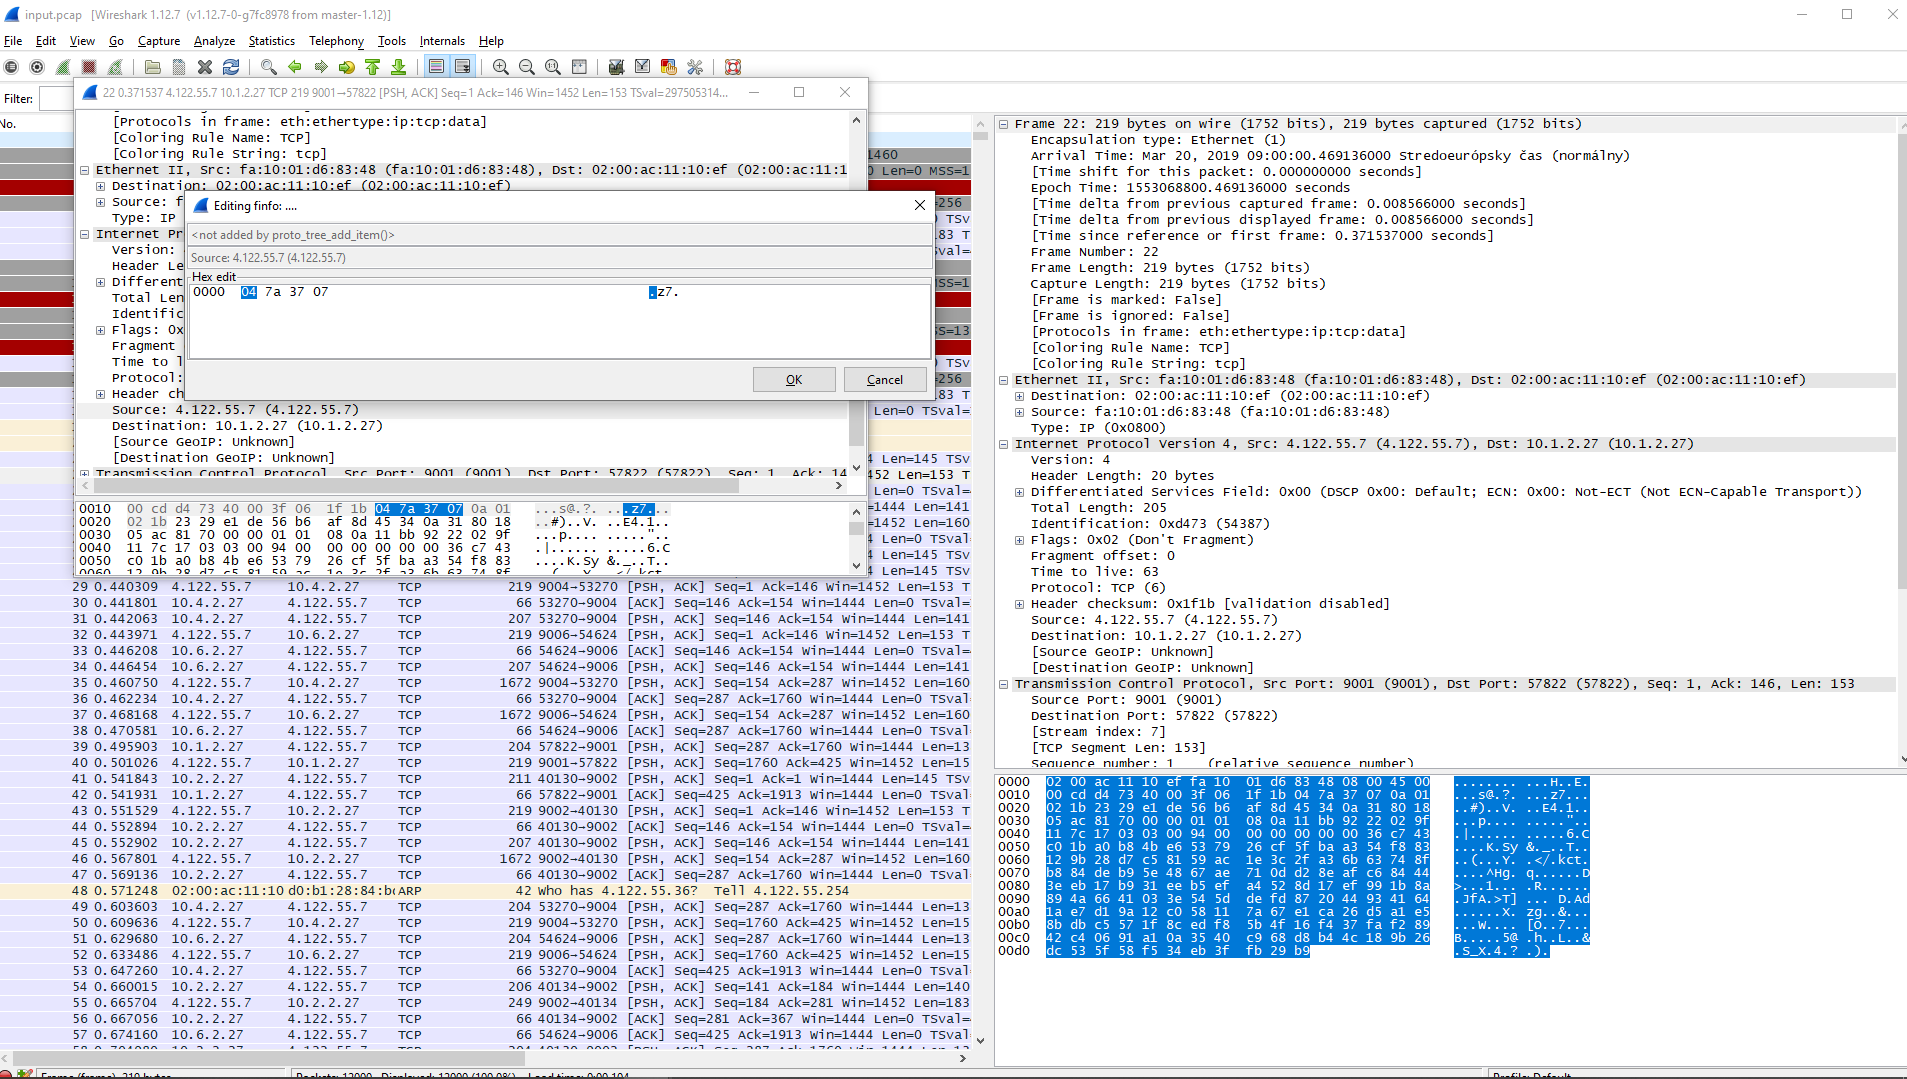
\includegraphics[width=0.9\textwidth]{images/wireshark_editing.png}
  \end{center}
  \caption{Editing in Wireshark v1.12.7}
  \label{fig:editwiresh}
\end{figure}

Another tool that provides GUI for packet field editing is Colasoft Packet Builder\footnote{\url{https://www.colasoft.com/packet_builder/}}, similar to earlier versions of Wireshark and brings automated checksum recalculation. However, bulk editing was again not supported. Colasoft Packet Builder supported creating new packets and inserting them into the packet capture file. This was done either by importing packets from different capture files or by crafting the packet in the GUI interface of the program. The GUI is shown in Figure \ref{fig:colasoft} sourced from the official Colasoft webpage.

\begin{figure}[h]
  \begin{center}
    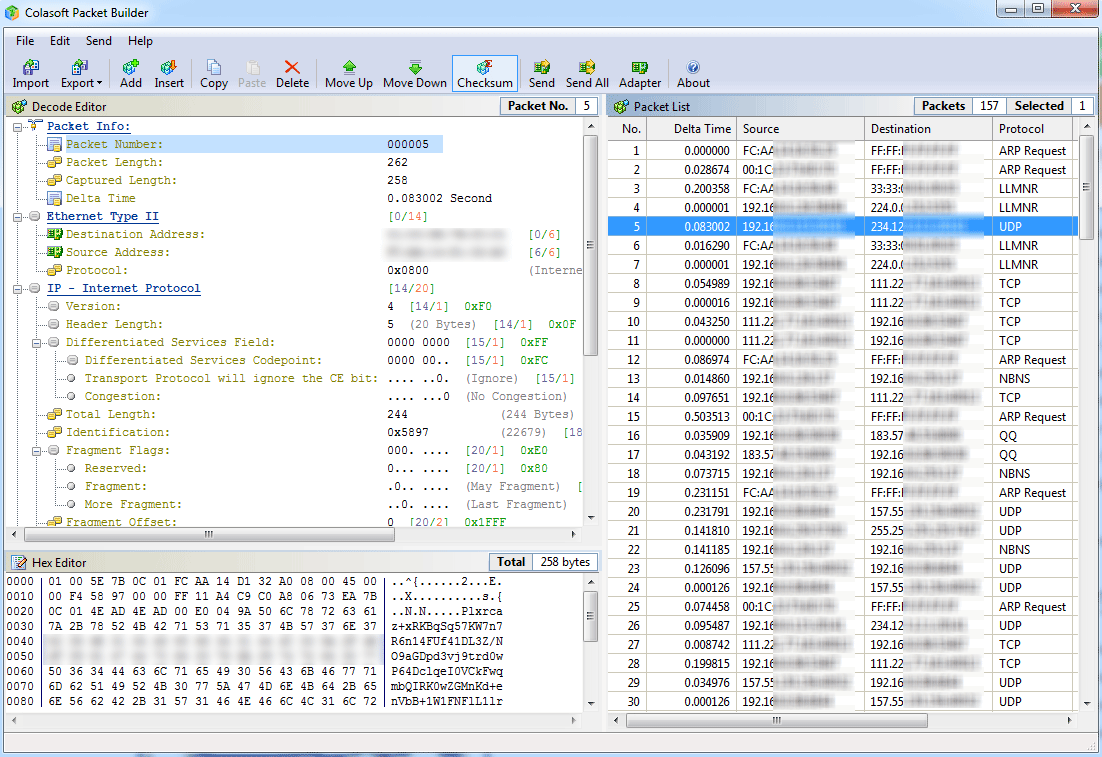
\includegraphics[width=0.9\textwidth]{images/colasoft.png}
  \end{center}
  \caption{Colasoft GUI}
  \label{fig:colasoft}
\end{figure}

There are also some paid versions of packet editors, like, for example, WireEdit\footnote{\url{https://omnipacket.com/wireedit}}, which brought support for bulk editing. Its steep price is, however, a~point to consider and means that only large organizations will be willing to invest in this software.

\newpage

\subsection{Command line tools}

Wireshark brings a~variety of command line tools\footnote{\url{https://www.wireshark.org/docs/wsug_html_chunked/AppTools.html}} that allow us to perform operations on PCAP(NG) files. Editcap allows removing packets from capture files as well as printing general info or splitting the capture, while Mergecap is a~tool that serves primarily to merge packets from multiple packet traces while ensuring correct packet order. Editcap can also be used to convert from one file format to another, for example, from PCAP to a~newer one PCAPNG as shown in the Listing \ref{lst:editcapform}, as well as reordering packets inside packet capture file as shown in the Listing \ref{lst:editcapreo}. As mentioned above, Mergecap is primarily used for merging files, but it has the ability to preserve relative timestamps or filter specific protocols while doing so. Mergecap usage is shown in the Listing \ref{lst:mergecap}.

\begin{lstlisting}[language=bash, caption={Changing the file format of capture file}, label={lst:editcapform}]
editcap -F pcapng input.pcap output.pcapng
\end{lstlisting}

\newpage

\begin{lstlisting}[language=bash, caption={Reorder packets inside a~capture file}, label={lst:editcapreo}]
editcap -o input.pcap output.pcap
\end{lstlisting}

\begin{lstlisting}[language=bash, caption={Merging capture files and preserving timestamps}, label={lst:mergecap}]
mergecap -aw output.pcap input1.pcap input2.pcap
\end{lstlisting}

Tcprewrite\footnote{\url{https://linux.die.net/man/1/tcprewrite}} does not come with wireshark but is rather a~Unix tool for complex packet trace manipulation that also allows bulk packet editing. It has the ability to recalculate checksum but does not offer the ability to edit application data. It is a~powerful tool that has the ability to alter packets fast and with many options available. It can modify the source IP address of all packets in the packet capture file as shown in the Listing \ref{lst:tcpmod} as well as truncate data in all packets of packet capture as shown in the Listing \ref{lst:tcptrunc}.

\begin{lstlisting}[language=bash, caption={Modify the source IP address of a~packet capture}, label={lst:tcpmod}]
tcprewrite --srcipmap=10.0.0.1:192.168.0.1 -i input.pcap -o output.pcap
\end{lstlisting}

\begin{lstlisting}[language=bash, caption={Truncate packet data in a~packet capture}, label={lst:tcptrunc}]
tcprewrite --truncate=100 -i input.pcap -o output.pcap
\end{lstlisting}

 One disadvantage with the tcprewrite lies within combining the filters and different modification options, which is not trivial and often requires the usage of cache files. Tcprewrite has a~huge potential and, as a~command line tool, can be used to automate the process while still being able to be called from programming languages like Python externally. This further extends their usage and potential.

\subsection{Programming libraries}

Programming libraries that allow packet editing bring a~higher level of automation and preserve the binary integrity of the data for the cost of higher user knowledge requirements. For example, Scapy\footnote{\url{https://github.com/secdev/scapy}} is a~powerful Python-based interactive packet manipulation program and library. It has the ability to craft packets as well as edit them on multiple layers while maintaining checksums and data integrity. Scapy can also be used to send packets to the network and listen on the network for incoming packets. Sniffing the network packets with scapy is relatively easy, and it is possible to customize the callback function in order to print just the info we are interested in. Listing \ref{lst:scapysniff} shows how network traffic could be sniffed. Notice the parameter \textit{iface}, which is, in fact, not necessary, as scapy listens on the main OS interface by default.

\begin{lstlisting}[language=python, caption={Sniffing network traffic}, label={lst:scapysniff}]
from scapy.all import *

def packet_callback(packet):
    print(packet.summary())

sniff(iface='eth0', prn=packet_callback)
\end{lstlisting}

As mentioned above, scapy also has the ability to send packets to the network. This is done by using the Scapy function \textit{send} after crafting the packet. An example is shown in the Listing \ref{lst:scapysend}.

\begin{lstlisting}[language=python, caption={Sending packets}, label={lst:scapysend}]
from scapy.all import *

packet = IP(dst="8.8.8.8")/ICMP()
send(packet)
\end{lstlisting}

Scapy also allows reading packet capture files. Packets that have been previously captured and saved for later analysis can be read with all the information as it was presented while the capturing took place, which is shown in the Listing \ref{lst:scapyread}.

\begin{lstlisting}[language=python, caption={Reading a~PCAP file}, label={lst:scapyread}]
from scapy.all import *

packets = rdpcap('packets.pcap')
for packet in packets:
    print(packet.summary())
\end{lstlisting}

Scapy is a~powerful Python library, and besides capturing and reading packets, it has the ability to manipulate their data. In addition to basic field manipulation, it is also able to manipulate different packet layers as well as raw data and payloads of packets. An example of packet modification is shown in the Listing \ref{lst:scapyman}.

\begin{lstlisting}[language=python, caption={Manipulating packets}, label={lst:scapyman}]
from scapy.all import *

packet = Ether()/IP(dst="8.8.8.8")/ICMP()
packet[IP].src = "192.168.1.1"
del packet[IP].ttl
\end{lstlisting}


\section{Associated risks}

When working with these kinds of tools that allow one to manipulate packet capture files, it is important to think about the associated risks with such actions~\cite{Messier2017-fz}. These may have a~high impact on the file itself as well as the ability to maintain data integrity and for the attacker to stay hidden. Especially manual tools, like direct hex editing, might corrupt the file irrecoverably, losing important capture data in the process.

Packet capture file corruption is just one type of risk that one goes through when editing packet captures. Other than that, it is possible to corrupt just a~packet itself in the packet capture file. This hugely depends on the type of tool used to modify such a~packet. Modifying packets with some tools also means that the checksum for different packet layers might be wrong because it does not get recalculated after the process of modification. Therefore, to predict these kinds of unnecessary issues, it is advised to use just the tools that do have the ability to maintain data integrity and also fix checksums. Attackers often choose these kinds of tools because it helps them to achieve the changes they are looking for without unnecessary overhead.

Packet capture files can often serve as a~piece of evidence for malicious acts. It is, therefore, important to ensure that the file is not corrupted and, while working with it, to do so carefully. Attackers may try to corrupt the file after the fact, even remotely, to clear their traces. Corrupting any information from the evidence might hinder the forensic investigation process.

\section{Prevention and impact}

It is important to think about the prevention of modification of captured data. As stated before, it may serve as an evidence of a~malicious act. Packet trace modification often refers to something that was unauthorized. Such unauthorized alteration of packet capture data can have significant implications for the security, privacy, and integrity of the network and the devices that are connected to it, with all the data flowing through the network as well. To prevent these kinds of packet trace modification, it is essential to implement effective security measures.

While talking about packet capture modifications, it is important to realize that packet capture is represented as a~file stored in a~computer or removable drive. This packet capture file then serves as evidence, and if this evidence is handed off from one person to another, the process must be documented. This process is often called the \textit{chain of custody}. Evidence of all kinds should be kept in a~protected location whenever possible. This is also true for packet capture. Documenting a~chain of custody is a~good strategy to make sure that the packet capture was not in contact with anybody who should not have access to the file in the first place.

\begin{itemize}
    \item \textbf{Encryption:} Usage of protocols that utilize encryption can help to protect the data transmitted over the network. It will be harder for the attacker to intercept specific data and modify them. 
    \item \textbf{Access control:} Access control should be implemented to limit who has access to network data and packet captures. Only authorized personnel should be able to access the packet traces.
    \item \textbf{Authentication:} Strong authentication mechanisms can help ensure that only authorized users are able to access packet traces.
\end{itemize}

The impact of packet trace modification can be more significant depending on the packet trace's role in the investigation. Packet traces can serve as critical evidence of malicious activity and should therefore be protected as any other evidence would be.

\begin{itemize}
    \item \textbf{Data loss or corruption:} Packet trace modification may lead to loss or corruption of network data, which can have significant implications for the integrity and reliability of the evidence part of the packet trace.
    \item \textbf{Security breaches:} Unauthorized modification to packet trace can provide attackers access to sensitive network information, potentially resulting in a~security breach.
    \item \textbf{Legal and regulatory compliance:} Packet trace modification can result in legal and regulatory compliance issues in industries with strict data protection regulations. This is especially the case with countries enforcing GDPR.
    \item \textbf{Financial loss:} Lastly, the impact of a~packet trace manipulation can result in financial problems causing loss of revenue or increased cost associated with remediation efforts.
\end{itemize}



\newpage
\chapter{Modification detection methods}
\label{chap:mdm}

In order to detect packet modification, it is important to understand the different detection methods available. They enable organizations to identify and prevent malicious attacks that could potentially compromise sensitive data. This chapter will explore various methods for detecting network packet modifications and discuss the limitations, false positives, and false negatives. By understanding the strengths and weaknesses of different detection methods, we can better understand network security and effectively detect and mitigate potential threads. The detection methods that will be discussed play a~huge role in Intrusion Detection Sytems~\cite{gtidaps}. IDS are systems that monitor network activity for malicious activities. Since the topic of offline modification detection is not particularly well documented, the text in this chapter relies on current methods of detection of live network traffic. Furthermore, it is perfectly fine to use the same methodology on offline packet captures in the form of PCAP(NG) files. While scanning the packets in the capture file, an application can be built that checks the packets for signatures and behavioral-based symptoms of modification and builds a~context about the capture. The application could then reconstruct the network sessions and perform detection methods.

Currently, we can divide the detection methods into three main groups:

\begin{enumerate}
    \item \textbf{Signature-based modification detection methods}
    \item \textbf{Anomaly-based modification detection methods}
    \item \textbf{Stateful protocol analysis methods}
\end{enumerate}

All of these have their use cases, different usages, and also positives and shortcomings, which will be discussed in this chapter. Understanding the different methods available and strategies used by these methods will help while thinking about designing detection methods in the following chapters of this thesis. This chapter will therefore provide an overview and an important foundation for further development of the detection script. Many of these methods provide a~basis for comparing against known types of attacks. Because the focus of this thesis is on the detection of packet modification, which the attacks are mostly based on, these methods can provide valuable insights into detection strategies.

The risk of false positives and false negatives is an important consideration. False positives occur when a~benign activity is mistakenly flagged as malicious. This could potentially lead to unnecessary alerts and increased workload needed to distinguish between them. False negatives, on the other hand, occur when a~malicious activity goes undetected by the intrusion detection system, either because the attack used a~new or modified signature or the system failed to recognize the signature due to a~configuration error. 

A deep description of different packets and protocols provided in Chapter \ref{chap:protocols} will provide an important baseline for understanding different types of detection methods. Understanding how the protocol works allows us to concentrate on the parts of the packet that actually matter and provides valuable insights into the protocol's inner workings.

\section{Signature-based modification detection methods}

In signature-based modification detection, the detection decisions are based on the knowledge of a~threat~\cite{LIAO201316}. It is the most widely used method for identifying potential security breaches. This method is essentially simple because it involves comparing network traffic against a~database of known signatures of malicious activity. These often consist of pre-defined patterns of data that indicate the presence of a~particular type of attack. Because of this, signature-based detection methods are often thought of as Knowledge-based methods. While analyzing the packet capture file, which contains a~snapshot of network activity over a~period of time, we can use many of the signature-based methods that apply to Intrusion Detection System methods.

Signature-based modification detection methods are usually effective in identifying known threats. These include viruses, worms, and Trojans. They have a~recognizable signature that can be detected and matched against a~signature database. This method is highly accurate and can detect known threats quickly and efficiently. In a~way, these methods work a~lot like antivirus systems in a~typical computer. While used in IDS, they work in the background processes. In order for them to work on \textit{offline} capture files, these methods have to be adjusted for packet captures. As stated in Section \ref{chap:protocols}, each protocol has different patterns and is used for different intentions. Some protocols carry \textit{payload}, and some do not. It is these properties that are valuable for signature-based modification detection methods because they can be verified against expected behavior. 

\textbf{Signature} in the signature-based modification detection methods refers to some kind of autograph of a~virus or malicious activity. One can think of them as a~fingerprint identifying specific attack method. Examples of such signatures can be as follows~\cite{gtidaps}:

\begin{itemize}[noitemsep,topsep=0pt]
    \item a~telnet attempt with a~username of root, which can be a~violation of an organization's security policy
    \item An operating system log entry that has a~status code e645. This could indicate that the host's auditing has been disabled.
    \item Email with .exe attachments are also a~common form of malware spread strategies.
\end{itemize}

Signature methods are the simplest form of detection because they compare activity against a~list of signatures using string comparison mechanisms. These technologies have little to no understanding of network protocols and can not directly track and understand the state of complex communication. They are unable to understand communication parties and can not distinguish between client and server, and are not able to form request-response pairs. They also do not build any context and, as such, lack the ability to remember previous data. These limitations further hinder their performance in detecting complex attacks that conform to multiple communication patterns~\cite{gtidaps}.

With signature-based modification detection methods, it is generally hard to keep the signatures and patterns up to date because it is time-consuming to maintain the knowledge. They are also highly ineffective against unknown and new types of evasion attacks~\cite{LIAO201316}.

These kinds of methods could be used to detect malware or scripts that might be run on the end device by hiding in the application layer data. Programming applications based on frameworks like Scapy could be used to verify each packet of the capture file and compare the payload of individual packets against a~known set of malicious commands and code snippets.

Generally, signature-based methods tend to have a~lower rate of false negatives since it is designed to detect known patterns of malicious activity specifically. If the signature database is up-to-date and comprehensive, the system should not have difficulty accurately detecting the most known threats. However, signature-based methods can have a~higher rate of false positives than any other detection method. This is particularly because of the configuration of sensitivity. Legitimate network traffic is then mistakenly flagged as malicious due to similarities with a~known signature. 


\section{Anomaly-based modification detection methods}

In order to detect threats that might go undetected in signature-based methods, anomaly-based modification detection methods were introduced as a~powerful method for identifying potential security breaches~\cite{gtidaps}. Anomaly-based methods involve analyzing network traffic for abnormal patterns and behavior that might indicate an intrusion rather than pre-defined signatures. Anomaly-based methods are particularly useful when detecting unknown or zero-day types of exploits. These are attacks that have not been previously observed and use new or unfamiliar tactics, making them difficult to detect using signatures. It is, therefore, important to have a~deep knowledge of different protocols and their expected behavior. For example, the Mac protocol mentioned in Section \ref{chap:mac} has a~different use and expected behavior than the IP protocol described in Section \ref{chap:ip}. Methods used in this type of detection build up profiles that represent normal behavior. This might consist of observing hosts, network connections, or application activity over a~period of time. 

Some of the major benefits of anomaly-based methods are the ability to detect new and unforeseen vulnerabilities, the independency of OS, and facilitating detection of privilege abuse~\cite{LIAO201316}. 

In order to be able to detect such vulnerabilities, a~profile for the network is built. An initial profile is generated over a~period of time, which is typically in a~range from hours to weeks, depending on the situation. This period is sometimes called a~training period, and it is also a~period during which the network is not protected. These profiles can be either static or dynamic. a~static profile is generated once and never changed afterward, while a~dynamic profile dynamically adjusts to the network changes. Because networks naturally change, a~static profile will eventually become so inaccurate that it will no longer provide satisfying protection. One huge problem with building profiles is that an attacker might already be attacking the network to some extent. This might mean that the profile would take such behavior as normal, and the attacker would be unrecognizable in the future. Profiles are then used to continuously scan the network for behavior that would be considered normal for a~given network like so~\cite{gtidaps}:

\begin{itemize}
    \item a~profile for a~network might comprise web activity an average of 13\% of network bandwidth. If this comprises significantly more bandwidth than expected, an alert might be sent to the network administrator alerting him of suspicious activity.
    \item a~profile for users might consist of emails sent per hour. If malware or any other threat would use emails to spread quickly around the network, it would be flagged as malicious activity.
\end{itemize}

As stated previously, unintentionally including malicious activity as a~part of a~profile is a~common problem with anomaly-based detection methods. Another problem is that a~weak profile accuracy due to consistent changes in the network might lead to more false positives. Benign activity that deviates significantly from the profile might trigger the alarm, especially in dynamic environments. These can occur when legitimate traffic is incorrectly identified as anomalous behavior, leading to unnecessary alerts and response measures. Anomaly-based methods are generally more resource-intensive, requiring significantly more computational power to analyze and interpret large numbers of network data. Another problem might be that huge amounts of computational power might be needed to build the profile correctly because the traffic and therefore computing activity on the network can be complex. Suppose a~particular maintenance activity occurs once per month. In that case, it might not be observed in the training period, or otherwise, it might be included in the profile, but the network is generally much calmer~\cite{gtidaps}~\cite{LIAO201316}.

Generally, when observing network activity in the packet trace file, all of the above-mentioned positives and negatives still apply, and the detection methods must account for the dynamic and sometimes unpredictable behavior of the network by adjusting sensitivity.


\section{Stateful protocol analysis}

Stateful protocol analysis is a~powerful method for detecting potential security breaches in network traffic. This method consists of analyzing the sequence and behavior of packets in a~network session to identify abnormal or suspicious activity. Being stateful, this analysis works by reconstructing the network session and analyzing the communication between client and server by building the context of communication and data exchanges. It is capable of understanding the network and its state, transport, application protocols, and many other indicators. These methods also work based on the fact that network protocols are usually well-described and can therefore be validated. To state an example~\cite{gtidaps}:

\begin{itemize}
    \item User starts a~File Transfer Protocol session. Initially, the session is in an unauthenticated state. Unauthenticated users are only allowed to perform a~few commands in this state, such as viewing help information or providing usernames and passwords to the server in order to verify their identity. While thinking stateful, it is important to understand the prospect of request-response that these protocols often work based on. Performing commands that are only allowed after the user is authenticated before he authenticates is considered suspicious.
\end{itemize}

The ability to know and trace the protocol states (e.q. pairing requests with replies) is something that makes these kinds of methods so powerful. Stateful protocol analysis often relies on vendor-developed generic profiles for specific protocols. These are generally based on protocol standards from the aforementioned RFCs and standard organizations like IETF~\cite{LIAO201316}.

Another strength of stateful protocol analysis lies in the ability to identify unexpected sequences of commands. These can vary from issuing the commands repeatedly or issuing the commands in a~different order than expected~\cite{gtidaps}. For example, a~DNS response should always be paired with a~DNS query, as well as TCP handshake should begin every TCP communication stream.

The protocol analysis performed by these methods usually consists of checking the reasonableness of the individual commands. This might mean checking command arguments against their maximum allowed length or checking that required command arguments are present, as well as undefined arguments that are present but should not be.

Unlike signature-based methods, stateful protocol analysis can detect zero-day attacks and advanced persistent threats which were not yet recognized or do not yet have recognizable signatures. Additionally, unlike anomaly-based detection methods, protocol analysis can provide detailed information about the attack, about what exactly was violated, and can therefore help quickly resolve and identify the issue.

On the other hand, statefulness means that these kinds of methods are usually more resource-intensive. They require significant computational power and memory to reconstruct network traces and sessions. Analysis can be a~complex task, requiring a~deep understanding of network protocols and the ability to distinguish between legitimate and malicious activity.

Another serious problem with stateful protocol analysis is that it is not able to detect attacks that do not directly violate the characteristics of generally acceptable protocol behavior. For example, some protocols can do many repeated actions in a~short period of time due to the unreachability of a~host, causing a~denial of service in the process. The interaction of different protocols and different implementations of protocols might also play a~role in the potential generation of false positives, which would generate unwanted alerts.

Despite all of the aforementioned challenges, stateful protocol analysis is one of the most important components of intrusion detection systems because of its ability to detect complex and evolving threats without clear signatures.

\section{Significance of understanding detection method properties}

All of the methods mentioned in this chapter, either signature-based, anomaly-based, or stateful protocol analysis, played a~huge role in deciding what detection methods to implement for the application part of this thesis. The characteristics of these methods directly influence what they can and can not detect. During the research of these methods, I analyzed all of the circumstances to come up with clearly defined detection methods that would be used to decide whether the packet capture file was or was not modified by any means.

By studying these methods, I gained a~deeper understanding of the mechanics of intrusion detection and the strengths and limitations of each approach. By leveraging the strengths of each method, it will now be easier to create a~system of modules in the detection application to detect the modifications to the packets. Even though the IDS is not part of this thesis, the core principles of modification detection methods provided an important foundation for developing modification detection methods in the application developed alongside this thesis. It is still possible to make use of signatures, as well as build a session context from a network packet capture. However, compared to IDS, there are some limitations. These include incompleteness of the packet capture and the possibility that the packet capture was modified. And the modification possibility is something that needs to be verified.

Throughout this chapter, I highlighted the key features of different methods, including the ability to detect specific know threats (signature-based methods), identify abnormal patterns or behavior (anomaly-based methods), and reconstruct network sessions to analyze packet behavior(stateful protocol analysis).

Overall, the study of these methods provided valuable insights into the complex nature of intrusion detection systems and the importance of combining multiple approaches to detect malicious acts. Recently shared research on the topic of packet modification methods~\cite{Howcanne5:online} has highlighted many ideas about how packet data could be modified. This paper has proven to be an important part of building the final application that would be used to detect these types of modifications on a~packet capture file.

\newpage
\chapter{Design and implementation of the proposed solution}
\label{chap:desimp}

The implemented application will aim to detect manipulation with the network traffic capture files and individual packet modifications with the intention to hide malicious acts in case of forensic investigation. These modifications and manipulations were deeply described in Section \ref{sec:manipul} and form a~strong basis for the application development and implementation of the solution. The final application should be able to read the packet capture file and present an analysis of this file based on implemented modification detection methods. The detection itself should be fully automated, with some specific configuration options still available, in order to tweak the application for user-specific needs.

The application's usage and configuration of some of the settings should be user-friendly, with minimum to no knowledge of programming languages. This can be achieved by dividing the application into modules and naming the specific configuration settings with self-explanatory terms.

The application will be able to process one or multiple packet captures and save a~log and results into specific files for further analysis. Application users will be able to turn specific functions and modules on or off, further tweaking the desired output to their specific needs.

After the analysis of the packet capture has proceeded, the application will present the final verdict as well as sub-results for each detection method so that the user can make a~verdict on his own as well.

The following Sections of this chapter will describe the technologies used to achieve this goal, the strategy for the application, and the detection methods implemented. This Chapter will also cover the application's architecture, configuration possibilities, structure, and the modules themselves, as well as statistical analysis of the packet capture file and the results the application represents.

\newpage

\section{Requirements and Design}

In order to create an application that would be capable of detecting modifications made to the packet capture file, it is important to have a~clear strategy before considering the architecture and design. The application aims to detect modifications made to packet capture and packets themselves. It is, therefore, safe to say that the target audience of this application will consist of network security professionals, network security enthusiasts, and analysts who need to ensure the integrity of packet capture files and the data they contain. Last but not least, the main goal of this application is to detect the changes made to packet traces, which may be a~legal document serving as proof or evidence of a~malicious act. Therefore, it must provide a~clear and concise way of expressing results in the form of statistics and probability of file modification.

To address the need to detect modification of packet captures, the application will utilize advanced algorithms and strategies to detect modifications made to packets inside PCAP(NG) files. The approach involves analyzing the contents of the PCAP(NG) file and comparing it to the standard behavior of packets on the network as well as building a~comprehensive context representing the file capture. Some algorithms can be used to check the packet directly, like making sure the checksum for the packet is correct, or the length of the packet makes sense; some algorithms need wider context. Therefore a~context representing the whole capture will be built. This will be done by utilizing a~database structure in the form of SQLite\footnote{\url{https://sqlite.org/}}.

One of the key challenges will be to ensure the accuracy and reliability of the detection methods and the representation of results. Given the nature of the network, it is not always possible to rely on standard concepts. Many factors might influence the final outcome, such as incomplete capture, custom protocol implementations, and others. The final result in the form of probability might, therefore, not be the only one to take in mind when considering the possibility of packet capture modification, and it might be on the end user to decide whether the results of one or the other modification detection method are more or less significant to him.

The strategy is to utilize Python\footnote{\url{https://www.python.org/}} as a~programming language of choice due to its complex capabilities, performance, and various open-source libraries and frameworks available. One of the key libraries that will be extensively used will be the program called Scapy\footnote{\url{https://scapy.readthedocs.io/en/latest/index.html}}\footnote{\url{https://github.com/secdev/scapy}}. Scapy also serves as a~Python library, which means it can be used alongside python code. This enables the application written in Python to directly interact with Scapy and utilize its capabilities, which consist of reading the packet capture, gathering data about packets, and even altering the packets. 

In summary, the application will provide a~way to analyze packet capture files and to gather detailed information about the behavior of the packets inside it, with clear and concise output that will represent the final probability and results for each modification detection method. The application will be able to be tweaked and run just the modification methods applicable or tweak the performance by utilizing multi-core data processing as well as logging and maintaining capture context.

\section{Architecture}

The application will be built upon Python programming language and a~library for parsing PCAP(NG) files called Scapy. In order to build a~context of the packet capture, the application will also utilize SQLite. More specifically, an SQL toolkit and Object Relational Mapper called SQLAlchemy\footnote{\url{https://www.sqlalchemy.org/}}. It is the interactions between these components that will allow the application to operate effectively.

The architecture of the application will consist of several components, including the main detector engine, configuration manager, database mapper, detection modules, and the user interface module, which provides statistical analysis.

The main detector engine is responsible for parsing the PCAP(NG) file and gathering basic information about the file. For this, the subprocess is called, which involves calling shell program \textit{capinfos}. After gathering essential information about file structure, its task is to start subprocesses that will be used for multiprocessing purposes and performance improvements. These subprocesses process packets one by one. This involves doing simple checks like making sure the checksum is correct and building up the context by putting the packets into a~queue in order to be saved to the database.

The detection engine is the core of the application. It ensures packets get processed and saved to the database. After processing all packets and saving them, detection modules are initialized and started one by one. The modules are divided by the layer of the TCP/IP model they operate on. From the link layer to the internet layer, the transport layer up to the application layer. Each module is responsible for providing analysis on the given layer by running multiple algorithms and methods to identify inconsistencies and anomalies in the packet capture data. These methods are applied to individual packets based on the context built by the database. After the detection methods are applied, statistical analysis is performed and probability is calculated. The output is directed either to the STDOUT or the HTML file.

\subsection{Technology stack}

In order to provide a~comprehensive analysis of the packet capture, the application incorporates various programming practices, programs, and libraries. These tools enable us to gain a~broader understanding of the context in which the packets were captured and any potential modifications that may have been made.


\subsubsection{Python}

The core of the application is built upon Python programming language. Python represents a~high-level programming language that is interpreted and was first released in 1991~\cite{lutz_2009}. Python was created by Guido van Rossum and has since become one of the most popular programming languages in the world.

One of the key features is the simplicity and ease of use. The syntax is designed to be clear and readable, making it an ideal choice for a~programming task of any means. Python offers a~large number of built-in data types and functions, and the number of libraries developed for Python is growing year by year.

Another key advantage of Python is its versatility. It can be used for a~variety of applications, such as web development to artificial intelligence. It has been especially welcomed in the mathematics community. It is easy to use because, as an interpreted language, it does not require a~compiler and is easy and fast to run.

Overall, the effectiveness, simplicity, and clear syntax with a~number of open-source libraries have played a~huge role in deciding to go with this programming language.

\subsubsection{Capinfos}

Another program that is utilized in the application is a~program called capinfos\footnote{\url{https://www.wireshark.org/docs/man-pages/capinfos.html}}. It is a~standalone program that comes installed with Wireshark and the ability to calculate the number of packets in the PCAP(NG) file as well as other information about capture length, byte flow, and others. It has been crucial in order to gather necessary PCAP(NG) file information before the analysis process begins. This program is called from the Python application using the subprocess function of Python, which runs the program and returns the output of capinfos to the Python application.

\subsubsection{Scapy}

To automatize the process of parsing PCAP(NG) files and to do so effectively, it is important to choose a~library that can extract the necessary information from the packet and analyze it.

While there surely are some limitations of the Scapy\footnote{\url{https://scapy.readthedocs.io/en/latest/index.html}} program, like its not full support for QUIC protocol, it has been the library of choice for Python-based networking applications for many years now.

Scapy exists as a~standalone program as well as a~Python library. It has the ability to craft packets, send them to the network as well as analyze PCAP(NG) files. It provides a~wide range of features for working with network packets, including capturing, decoding, and manipulating packets in real time. It supports many protocols and packet types, such as Ethernet, TCP, UDP, DNS, and others.

One of the key features is the ability to edit packets as well as replay them to the networks or even craft new packets. These crafted packets can then be injected into the network. Scapy has also been extensively used while preparing the dataset for testing purposes of the application created for this master's thesis. With its ability to directly manipulate even the application layer and payload of packets, it has been a~great tool to use for these kinds of purposes. Scapy was also extensively used in dissecting packets into specific layers and information needed to build the context of the packet capture file as well as performing basic tests for checksums and packet lengths.

\subsubsection{SQLAlchemy}

The context of the packet capture file is represented in a~database file. In order to save the data from Scapy to a~database file, the application utilizes the SQLAlchemy\footnote{\url{https://www.sqlalchemy.org/}} Python toolkit. SQLAlchemy provides a~simple way to generate SQLite databases and many others. It allows us to create tables with relations and to utilize ORM capabilities. This allows simple workflow and straightforward manipulation of the database as well as gathering the information from the database using filters.

\subsection{Data retrieval and data storage}
\label{sec:ds}

The application retrieves all the data from the input PCAP(NG) file using a~combination of capinfos and Scapy. Upon running the application, the essential data about the PCAP(NG) file are collected using capinfos, and the PCAP(NG) file is therefore verified to be a~valid packet capture file. The output of capinfos is parsed in Python into a~dictionary of packet file attributes and values. These can be later used, for example, for estimating the time left until the packet processing ends.

After capinfos reads the necessary data from the PCAP(NG) file, the process of packet capture analysis begins. The packets are inserted into queues, one for individual packet processing and one for building the context using SQLAlchemy and an SQLite database. The database contains two tables, \textit{Pcap} table, which consists of the following:

\begin{itemize}[noitemsep,topsep=0pt]
    \item \textbf{id\_pcap}: ID that represents a~PCAP file's unique ID in case the program is run on a~dataset of multiple PCAPs.
    \item \textbf{path}: Path to the PCAP(NG) file.
    \item \textbf{packets}: Relationship that is used to retrieve packets from the Packet table that belong to this PCAP(NG) file.
\end{itemize}

And the \textit{Packet} table that contains information about the packets themselves consists of the following:

\begin{itemize}[noitemsep,topsep=0pt]
    \item \textbf{id\_packet}: Unique ID representing given packet
    \item \textbf{packet\_timestamp}: Timestamp of the packet
    \item \textbf{type}: Packet type, either Ether or IP
    \item \textbf{protocol}: Protocol of the packet
    \item \textbf{ip\_src}: Source IP address
    \item \textbf{ip\_dst}: Destination IP address
    \item \textbf{port\_src}: Source port
    \item \textbf{port\_dst}: Destination port
    \item \textbf{seq}: Seq number of TCP stream packet
    \item \textbf{ack}: Ack number of TCP stream packet
    \item \textbf{tcp\_segment\_len}: Length of TCP segment in given TCP packet
    \item \textbf{tcp\_flags}: TCP flags
    \item \textbf{window}: TCP window
    \item \textbf{eth\_src}: Source MAC address
    \item \textbf{eth\_dst}: Destination MAC address
    \item \textbf{dns}: DNS data
    \item \textbf{arp\_op}: ARP op code
    \item \textbf{arp\_ip\_src}: ARP source IP address
    \item \textbf{arp\_ip\_dst}: ARP destination IP address
    \item \textbf{ttl}: IP header Time To Live property
    \item \textbf{mss}: TCP header maximum segment size
    \item \textbf{tls\_msg\_type}: TLS message type
    \item \textbf{tls\_ciphers}: Ciphers in given TLS packet
    \item \textbf{dhcp\_yiaddr}: DHCP IP address
    \item \textbf{icmp\_type}: Type of ICMP packet
    \item \textbf{user\_agent}: User-agent of HTTP packet
    \item \textbf{ip\_flag}: IP flag
    \item \textbf{ip\_fragment\_offset}: Fragment offset of IP packet
    \item \textbf{ip\_identification}: IP identification
    \item \textbf{length}: Length of packet
    \item \textbf{is\_ftp}: True if the packet is detected as an FTP packet
    \item \textbf{id\_pcap}: id of the PCAP(NG) that the packet belongs to
    \item \textbf{pcap}: Relationship representing the relationship between Pcap table and Packet table
\end{itemize}

The data from the database are queried for the specific methods in the way that the specific method expects them, and only the necessary packets are retrieved each time, ensuring the performance of the application.

\section{Application structure}

Structuring the application into multiple modules ensures scalability and inadvertently makes it easier to manage while maintaining clear code structure and separation on a~logical level. Therefore, the application is divided into modules. The main application engine imports these modules and calls their functions based on the configuration file and input parameters. The parameters and the configuration file further tweak the application and its output. The core functionality of the application is always preserved.

\subsection{Input parameters and configuration}
\label{sec:config}

It is possible to tweak the application, the desired output, and the application behavior in two different ways. Firstly, let us consider the configuration file, which is required for the application to run properly and utilize different behavioral as well as functional parameters.

The configuration file is based on the YAML\footnote{\url{https://yaml.org/}} structure. YAML represents a~human-friendly data serialization language popular among many programming languages, Python included. It is easy to read for humans as well as for programming languages, and it accomplishes the task of configuring different application behavior based on setting property values.

The configuration itself can be used to configure application behavior in terms of performance as well as execution of specific test suites, and the properties of the configuration file are described below:

\begin{itemize}[noitemsep,topsep=0pt]
    \item \textbf{database}:
        \begin{itemize}[noitemsep,topsep=0pt]
            \item \textbf{engine}: The database engine used by the application. It should be set to SQLite.
            \item \textbf{file}: The file name created by the database engine.
        \end{itemize}
    \item \textbf{app}: 
        \begin{itemize}[noitemsep,topsep=0pt]
            \item \textbf{chunk\_size}: The number of packets to be processed into the database in one chunk.
            \item \textbf{buffer\_multiplier}: Multiplier for the buffer size, memory, and speed-related setting.
            \item \textbf{ntp\_timestamp\_threshold}: Threshold difference between NTP timestamp and packet timestamp.
            \item \textbf{check\_last\_bytes}: Check last [x] bytes of the packet payload for validity.
            \item \textbf{allowed\_communication\_silence}: Allow communication silence for a~given IP address in seconds.
            \item \textbf{allowed\_latency\_inconsistency}: Allow latency difference to be more than [x] times different.
            \item \textbf{workers}: Number of process workers. Leaving this empty will use all available system cores.
            \item \textbf{custom\_private\_network}: Custom private network setting, in case the private network is not in the usual range.
        \end{itemize}
    \item \textbf{tests}:
        \begin{itemize}[noitemsep,topsep=0pt]
            \item \textbf{pcap}: Turns on or off PCAP(NG) specific tests
            \item \textbf{misc}: Turns on or off packet specific tests
            \item \textbf{link\_layer}: Turns on or off Link Layer tests
            \item \textbf{internet\_layer}: Turns on or off Internet Layer tests
            \item \textbf{transport\_layer}: Turns on or off Transport Layer tests
            \item \textbf{application\_layer}: Turns on or off Application Layer tests
        \end{itemize}
\end{itemize}

The configuration file is a~required part of the application and ensures that the application will behave as expected to user-specific needs.

Another possible configuration is by utilizing application-specific arguments that are specified in the command that runs the application. This can be done by different options available as command line arguments. The arguments available are the following:

\begin{itemize}[noitemsep,topsep=0pt]
    \item \textbf{-c / --config}: Represents the path to the configuration file. If this argument is not specified, the default config.yml file is used. In case the file does not exist, is corrupted, or does not have the expected structure, the program ends.
    \item \textbf{-l / --log}: Specifies the log level for the application. Different log levels display different messages on the STDOUT while the application is running and processing packets.
    \item \textbf{-o / --outputhtml}: After the application ends, this argument specifies whether the results of modification detection should be written to the output HTML file. If yes, the HTML file is created after the application ends with the specific file name as an output name. The file consists of results and a~summary of modification detection.
    \item \textbf{-f / --filelog}: Turns on logging to the log.log file in the current directory.
    \item \textbf{-i / --input\_pcap}: Specifies input packet capture file to be processed.
    \item \textbf{-d / --dataset\_dir}: Specifies a~directory with packet capture files that should be processed. In this case, a~directory is traversed, and the application is run for each PCAP(NG) file found in the given directory.
\end{itemize}

Note that the \textit{-i} and \textit{-d} parameters are mutually exclusive. This means that one and only one should be present at a~time.

\medskip

The configuration correctness is checked in the Config class. This module ensures that the arguments provided are correct and that the configuration file is properly formatted YAML style file.

\subsection{Main application engine}

After the application is initialized and the configuration is verified, the main application engine starts by saving the necessary PCAP(NG) information to the database table. After this, a~function called \textit{check\_pcap} is executed. This function first initializes the necessary components, queues, and processes. It then proceeds by reading the packet capture packet by packet and puts these packets into the queues. Processes that were started await the packets in the queues, and as soon as the packet gets into the queue, it is expected to be processed soon. The processes are divided into two worker groups as follows:

\begin{itemize}
    \item \textbf{Process worker group}: This worker group manages simple packet-by-packet detection checks, like making sure the checksum and packet lengths are correct.
    \item \textbf{Saving worker group}: This worker group contains one worker that is responsible for parsing the packet and saving necessary information to the database. This is essential for the full capture context to be built.
\end{itemize}

As soon as the last packet is put into the queue, the application waits for all worker groups to finish. Process workers share a variable, which is used to increment the necessary counters for packet-based modifications. This is done by sharing a~dictionary using \textit{multiprocessing.Manager()}, which takes care of sharing the results list across worker groups. The synchronization is done by utilizing locks.

The application then proceeds to execute different tests on the whole packet capture context. These tests are divided into modules, which will be described in the following subsection.

The tests that have been allowed in the configuration file are run, and the results are again accumulated after all of the testing procedures end. For this, the \textit{pcap\_modifications} and \textit{packet\_modifications} Python dictionaries were created. These hold the overall results of the modification detection, which are then forwarded to the Statistics module. This module will be further described in Section \ref{sec:res}.

\subsection{Modules}

Modules represent the main logic of the application, which is modification detection. The detection methods have been divided into these modules based on the scope they operate on. Additionally to these modules, there is a~\textit{Functions} module, which serves as a~helper module for the aforementioned modules. The Functions module provides helper functions like checking if the specific IP is a~private IP or providing some complex filtering on the database queries.

\subsubsection{Database module}

The database module takes care of creating the database file and the context of database tables. The database has two tables, \textit{Pcap} and \textit{Packet}, which were deeply described in Section \ref{sec:ds}. The database module further handles the process of saving PCAP-specific information like PCAP(NG) path and ID to the Pcap table, as well as packet-specific information parsed using Scapy into the Packet table, in order to build the context of the packet capture.

\subsubsection{PcapData module}

In order to check the basic information from the PCAP(NG) file header, the PcapData module provides a~clear interface that provides detection methods for the PCAP(NG) file itself.

\subsubsection{Miscellaneous module}

The miscellaneous module provides detection methods specific to packet-related analysis. These include checksums, packet lengths, and other packet-specific information that does not need context in order to be verified.

\subsubsection{LinkLayer module}

LinkLayer module provides modification detection methods for Link Layer-related anomalies and mismatches. Having the full context of the whole packet capture ensures that the module will have all the necessary data available.

\subsubsection{InternetLayer module}

Similarly to the LinkLayer module, the InternetLayer module offers modification detection methods for the Internet layer-specific packet information.

\subsubsection{TransportLayer module}

The TransportLayer module includes modification detection methods related to the TCP/IP Transport Layer.

\subsubsection{ApplicationLayer module}

The last layer of TCP/IP model is the Application Layer, and the ApplicationLayer module offers modification detection methods specific to this layer.


\section{Implemented detection methods}

The modules described above contain the modification detection methods that were implemented in order to detect the modifications made to PCAP(NG) files as well as packets themselves. The methods implemented in these modules play a~huge role in the deciding factor, as the sum of their results, the weighted average, and statistical analysis that will be described in Section \ref{sec:res} result in the final resulting probability of the packet capture modification. All of the different detection methods implemented will be described in the subsections of this section. The detection methods and algorithms developed to detect network packet trace modifications are based on Chapter \ref{chap:mdm}, which built an important foundation with the modification detection approaches described. Many of the detection methods are also based on recent research on this topic~\cite{Howcanne5:online}, which provides many modification ideas. Many modification detection methods originate from the ideas and suggested approaches on how to detect them from this research paper.

\subsection{Packet capture file analysis}

Packet capture file analysis implemented in the module PcapData contains two major detection methods:

\subsubsection{Checking the snapshot length context}

This detection method establishes the PCAP(NG) snapshot length limit from the PCAP(NG) file global header gathered through capinfos. After that, this method checks all of the packets and builds a~snapshot length context. This is then compared, ensuring that the number correlates and there are no suspicious constants like that one length would be more than 50\% of the packet trace, indicating that the snapshot length was either not set correctly or that the packets were truncated.

\subsubsection{Checking the file and data size}

The file size of the packet capture should always be higher than the data size. In case the data size is higher, it means that the packets were malformed or truncated and that the data is missing.

\subsection{Packet-based detection methods}

Modification detection methods that are able to be performed on a~single packet without a~context are essential because they tell us about the packet structure itself. If the packet was manipulated in any way, the checksum could be incorrect, or one of the lengths could be mismatched. Therefore, the Miscellaneous module implements the following detection methods.

\subsubsection{Checking ports and protocols}

Each protocol has standard ports that it uses. Usage of nonstandard protocols is, however, pretty common. Some applications might use specific implementations of protocols that use nonstandard ports, and it might get flagged as suspicious during this modification detection method. The list of standard ports for protocols was gathered from IANA\footnote{\url{https://www.iana.org/assignments/service-names-port-numbers/service-names-port-numbers.xhtml}}.

\subsubsection{Checking checksums}

Checksums are essential because they tell us whether the packet or its contents were manipulated directly, as the hash value the checksums represent will be incorrect. This detection method verifies TCP, UDP, IP, and ICMP checksums by storing the original value and recalculating it. However, it is often common for the checksums to be incorrect while the packet is still fine. This is due to the checksum offloading that could be taking place\footnote{\url{https://wiki.wireshark.org/CaptureSetup/Offloading}}.

\subsubsection{Verifying the packet length}

Each layer and subsequent payloads have defined lengths. These lengths should correlate to the packet length, and the different lengths of the layers should always add up to the same length, as well as the payloads.

\subsubsection{Scanning the packet payload}

If the payload was malformed or manipulated in such a~way that the padding of 0s was added to the payload end or any other random characters, it should be clearly visible from the packet payload.

\subsubsection{Confirming the frame wire length and packet length}

If the packet's length on the wire does not match the length in the packet capture, it might mean the packet was malformed or truncated.

\subsubsection{Checking mismatched NTP timestamp}

If the NTP sent timestamp does not correlate with the timestamp that the packet was sent on, it might mean that the packet was injected or manipulated.


\subsection{Link Layer detection methods}

Link Layer detection methods verify the Link Layer protocols and properties in the packets for modification and manipulation. These mostly consist of MAC address and ARP-based checks.

\subsubsection{Inconsistent MACs and IP addresses}

One MAC address should have one IP address, and while there are valid reasons why this might not be the case, in general, it is not that common. If more IP addresses are assigned to one MAC address, it indicates possible malicious acts.

\subsubsection{Missing ARP traffic}

If communication occurs on the network, and the TCP or UDP traffic is present, ARP traffic for the same MAC address should also be present.

\subsubsection{Lost ARP traffic}

Similar to the previous detection method, if the MAC address is present in the ARP traffic, it should also be present in other traffic as well.

\subsubsection{Missing ARP responses}

If an ARP request is generated, there should be an ARP response coming from the requested machine. If there are no responses to the requests, it might indicate that some traffic was removed or that the requests were injected. However, this kind of behavior is still considered acceptable on the network.

\subsection{Internet Layer detection methods}

Internet Layer detection methods are part of the InternetLayer detection module. The core strategy of this module and its detection methods is to focus on the IP protocol.

\subsubsection{TTL inconsistency}

The IP header contains multiple fields. One of them is the TTL field. This field indicates the hop limit between the two communication parties. This should be the same across all communications between the two IP addresses. For accuracy, this is only checked on the SYN TCP packets.

\subsubsection{Inconsistent fragmentation}

Fragmentation is checked and verified by IP identification numbers. IP packets with the same IP ID indicate they should belong to each. Fragmented IP packets have the IP ID always the same. However, sometimes this can be ignored, and some implementations of QUIC protocol do not rely on this number at all, hindering the detection process of this method.

\subsubsection{Sudden drop in traffic}

If there is a~sudden drop in communication between two communication parties, it could indicate that some of the traffic was removed.

\subsection{Transport Layer detection methods}

In the TransportLayer module, the detection methods focus on the TCP and SSL/TLS protocols in order to check for inconsistencies.

\subsubsection{Inconsistent interpacket gaps}

We can check the first round trip time of SYN and SYN-ACK packets and later compare the round trip times against other TCP handshakes for the same communication. The round trip time should be the same, without any big deviation.

\subsubsection{Incomplete TCP streams}

By checking for SYN and SYN-ACK packets, we can get an idea about the TCP stream and if the handshake took place, indicating that the connection is established. Streams without the three-way handshake are considered to be incomplete. However, this is pretty common at the start of the packet capture.

\subsubsection{Inconsistent Maximum Segment Size values}

In case the Maximum Segment Size value changes in one communication, it is considered suspicious, as the value should not change for one communication channel. Again, for improved accuracy, we are only checking the SYN packets.

\subsubsection{Inconsistent Window size values}

The TCP Window size field represents the flow of the data. This value should be the same for all SYN packets in a~single communication stream.

\subsubsection{Mismatched TLS ciphersuite}

If the cipher suite offered by the TLS client during the Client Hello TLS traffic changes, it is considered suspicious. The cipher suite offered should not have a~reason to change dramatically during one communication.


\subsection{Application Layer detection methods}

The Application Layer of the TCP/IP model covers multiple protocols like DNS, HTTP, and others. The behavior of these can be verified and compared to other traffic in the packet capture. If there are inconsistencies or mismatches, it can identify manipulated packet captures.

\subsubsection{Translation of unvisited domains}

In case a~domain is translated using DNS and IP address is returned, this address is expected to be visited, with traffic being present in the packet capture. However, sometimes it is quite common for web browsers to cache the answers or pre-request them.

\subsubsection{Incomplete FTP}

Similarly to incomplete TCP, we can check for FTP completeness for example, by checking if the three-way handshake took place and later if both port 20 and 21 were used for communication, as port 21 is used for control messages and port 20 for data stream.

\subsubsection{Verify DNS query}

Both DNS queries and responses carry a~DNS query name, which should be the same for one DNS pair. If this is not the case, it is safe to say that the packet trace has been manipulated.

\subsubsection{Mismatched DNS answer stack}

As DNS servers sometimes query other servers in the case of CNAME records, the records and queries in the DNS answer stack should be the same. Changing one of the records will result in a~mismatched DNS answer stack.

\subsubsection{Missing translation of visited domain}

In order to access a~website, we need the IP address. We can get the IP address of the website using DNS. However, if we have traffic where no IPs were translated using DNS, it can be considered suspicious. Some computers and browsers cache the translations, and the IP addresses of local computers are translated using ARP. This can influence the final outcome of this detection method.

\subsubsection{Missing DHCP IPs}

If an IP address is present in a~DHCP traffic, it should also appear in other connections.

\subsubsection{Missing ICMP IPs}

If an IP address is present in an ICMP traffic, it should also appear in other connections.

\subsubsection{Inconsistent user agent}

The user agent with which the computer communicates with other communicating parties should be the same for a~triplet of source and destination IP addresses and a~port. If this is not the case, the packet trace was most likely manipulated in order to cover the user agent traces.

\newpage

\section{Results processing}
\label{sec:res}

The results from the modification detection methods run by the application are printed on the standard output stream (Stdout) by default. This behavior can be modified by the command line arguments, as described in Section \ref{sec:config}. The application is able to generate the results in the form of an HTML file, which provides a~clear overview of the results of the modification detection methods.

It is important to understand the results and what exactly they represent. Therefore, for clarity and accuracy, the results are always contextual. This means that they are always in the same format but focused on the type of property they try to detect. In the case of individual packet analysis, the packet mismatch is put into a~ratio against all of the packets in the trace file. Similarly, in the case of TCP stream detection, the number of failed TCP streams is put into a~ratio against the number of TCP streams. 

Each detection method has been given a~category, based on which the final resulting probability of the packet capture modification is calculated. Some properties, like checksums, are not really reliable, and therefore it is not wise to make any major assumptions based on just the checksum correctness. However, they still do play a~role. On the other hand, malforming the packets, or manipulating the DNS queries, plays a~much bigger role in the deciding factor and has a~higher weight when calculating the final modification probability.

However, it is not possible to predict the preferences and priorities of the final user. Therefore, the final outcome should serve as a~theoretical possibility that the packet capture was modified. The end-user of the application can give higher priority to the checksum part, as the network status and behavior could be different for some specific implementations. The results can be interpreted in many ways, and it is not wise to rely only on the resulting percentage probability provided by the application but rather to understand the various test cases and the properties they verify.

\subsection{Output format}

The output format of the application is, by default, the standard output stream. The application allows the logging of major events, like the stage of the detection process and the estimated time left until all packets are processed. Depending on the log level selected by the command line arguments, the level of information printed can change. 

In general, the processed filename as well as current progress and results, are always displayed. Results are printed with a~\textbf{Result} text as a~header, with PCAP-specific and packet-specific detections separated. Each detection method was given a~friendly name that should describe it for the end-user clearly.

In the case of the standard output stream, the results are displayed and then the final probability of the modification is displayed as a~percentage, with the total processing time of the given file printed below. In the case of HTML output, the standard output is still generated. In addition, the HTML file structured as multiple HTML tables with basic styling is also generated in the root folder of the application. This file is given a~name after the input file name followed by a~string \textit{results} and a~standard HTML file extension in this format \texttt{\_\_\_results.html}. The resulting HTML file is structured into three tables, with the first two being the results of PCAP(NG) modifications and packet modifications, respectively, and the last one being the overall summary of the detection with the final percentage probability.

\subsection{Understanding the statistical analysis and final outcome}

Each result from the detection method is calculated in the detection method itself because each detection method provides the number of packets, pairs, or streams that failed the detection and are considered suspicious. These numbers are then returned, and a~context of all detections is built. This context of PCAP(NG) and packet detection results is then forwarded to the Statistics module, which handles calculating the final statistical probability that the packet trace was manipulated. However, it is still important to understand the sub-results that lead to this calculation. They can play a~different role for a~different end-user who might give the priorities to modification detection of methods that are not significant.

The calculation of the final probability is done using the Logistic function~\cite{doi:10.1021/j150299a014}. The Logistic function is commonly used in various fields ranging from biology to mathematics. It can also be used for logistic regression, which is a~statistical model used for binary classification problems, where the goal is to predict the probability of an event. This function can further be represented as shown in Equation \ref{eq:stat}.

\begin{equation}
\label{eq:stat}
f(x) = \frac{L}{1 + e^{-k(x - x_{0})}}
\end{equation}

Where 

\begin{itemize}[noitemsep,topsep=0pt]
    \item \textbf{L} is the supremum of the values of the function
    \item \textbf{e} is Euler's number
    \item \textbf{k} is the logistic growth rate
    \item \textbf{x\textsubscript{0}} is the value of the function's midpoint
\end{itemize}

It is important to choose the values of the function according to the results we expect and according to the significance of the results. The supremum of the values, \textit{L} in our case is 100, the value of \textit{k} was chosen as 0.15, and the \textit{x\textsubscript{0}} was given a~value of 10. These values influence the final value of the detection probability and will play a~huge role in the testing and evaluation described in Chapter \ref{chap:testing}. The choice for these values was done practically, by confronting and observing the results. The values were tweaked to match the significance of the modification and to show the slightest changes in a~clear way.

Overall, the resulting probability of modification will serve more as a~guide for the end user than a~final, static probability value. The network and the behavior of some protocols may sometimes vary, depending on the protocol's specific implementation. The end-user might prioritize various aspects of the detection, like checksums or ports, which are not prioritized by default. This might influence the real output of the results, which can be interpreted differently.


\newpage
\chapter{Testing and evaluation}
\label{chap:testing}

Application testing and result evaluation are an important part of every application development. It reveals the accuracy and verifies that the application does what it is supposed to do. Therefore, this chapter will consult the testing methodology and the evaluation of the results. This will help us understand the shortcomings of the proposed solution, as well as highlight the key strengths and weaknesses.

\section{Testing environment}

In order to test the application thoroughly, the testing was done on a Linux operating system, specifically Linux Manjaro. The system had 16GB of RAM and the processor was the Intel Core i7-8550U. The Python version was 3.8.10, and the specific versions of external modules are described in the README of the application. As the application is written in Python programming language, the prerequisites can be installed using Python package manager pip\footnote{\url{https://pypi.org/project/pip/}}. The prerequisites are also stored in the \texttt{requirements.txt} file for easier installation.

\section{Creating the dataset}

In order to test the detection methods implemented in the proposed solution, a~test set consisting of multiple packet capture examples needs to be created and verified. The methods of manipulating the packet captures were profoundly described in Chapter \ref{chap:modif}, and to automate the process, the programming libraries were preferred.

Python was chosen as a~programming language of choice, with the Scapy library as well as the Tcprewrite program used by the Python script directly. The baseline packet capture was provided by the Masaryk University Cybersecurity research group and is based on this article~\cite{TOVARNAK2020105784}. It has a size of 9379 kB and contains exactly 12000 packets. The capture duration is 77.900059 seconds with a data byte rate of 117 kBps. The average packet size is 765.65 bytes, and the average packet rate is 154 packets per second. This network packet capture was captured with 65534 bytes capture length with a time ranging from \texttt{2019-03-20 09:00:00.097599} to \texttt{2019-03-20 09:01:17.997658}.

\subsection{Dataset script}

The script to generate the examples of modified packet captures utilizes the Tcprewrite program as well as the Scapy library. This is in order to generate modified packet captures that will later be tested by the main application. The script can be run directly, and it will use the provided example packet capture by default, as well as generate the modified packet captures to the \texttt{/dataset} directory. Every generated packet capture will have a~default prefix \texttt{pacp\_output\_} with an index of the modification. This basic configuration can be modified in the script's global variables section.

After running the script, it first checks if the input file and the directory for the output files exist. In case the input file does not exist, the script will end prematurely. In case the directory does not exist, it gets created. If the directory already contains any files, these get purged in the process.

Subsequently, the provided example packet capture is loaded. The script then starts generating the modified examples of packet capture using the Tcprewrite. After the initial examples using Tcprewrite are generated, the script runs three variants of modifications by the Scapy library. First, the basic modifications are generated. This involves changing MAC addresses, randomizing IP addresses, and others. The second set of generated packet captures targets specific detection methods implemented in the main detection application. These include DNS modifications, ARP manipulation, and others. Lastly, more advanced packet trace examples are generated, utilizing multiple modifications and trace manipulation.

The script informs about every packet capture file generated with a~simple informative message containing basic information about what modifications were done. This is done so that the end user has a~general overview of the generated packet traces.

After the script ends, the output directory information is displayed, informing the user about successful completion and that the example packet captures were generated.

\subsection{Generated packet captures}

The script that takes care of generating samples of modified packet captures generates a~total of 30 modified PCAP files. The baseline file has around 9MB, and the size of generated modified packet captures ranges from a couple of KB to 9MB. The strategy is to generate packet captures with multiple levels of modification to show the strengths and weaknesses of the main application and the ability to detect these changes. The script generates packet captures with slight changes, like changing the IP address of the source or destination host or randomizing the MAC addresses. These are usually harder to detect because they may not affect the whole trace file or might affect properties with lower priorities. Another type of generated packet capture is targeted toward the specific detection methods implemented, like DNS modification detection, ARP traffic manipulation, and others. The last category represents more advanced changes made to the packet captures, such as changing multiple values and layers at once and modifying payloads. This might show more significant results, as the detection result is based on the average of the detection methods. The modified packet captures are described in the \texttt{docs/results.html} file. This file, which is also present in the attached archive, contains the modification information for a~specific generated file, as well as the overall result for the file.

\section{Dataset testing evaluation}

In order to properly test all of the generated dataset files, it is crucial to generate the dataset using the command shown in the Listing \ref{lst:ds}:

\begin{lstlisting}[language=bash, caption={Generate the dataset files}, label={lst:ds}]
python src/createdataset.py
\end{lstlisting}

After the dataset files were generated, we can execute the main application on this dataset, using the command shown in the Listing \ref{lst:main}:

\begin{lstlisting}[language=bash, caption={Run the main application on the dataset}, label={lst:main}]
python main.py --dataset ./dataset
\end{lstlisting}

\begin{table}[]
\begin{tabular}{lll}
\hline
\textbf{Input file}                                & \textbf{Total time}                & \textbf{Result} \\ \hline
\multicolumn{1}{l|}{dataset/pcap\_output\_01.pcap} & \multicolumn{1}{l|}{14.07 seconds} & 30.31\%         \\
\multicolumn{1}{l|}{dataset/pcap\_output\_02.pcap} & \multicolumn{1}{l|}{27.09 seconds} & 38.05\%         \\
\multicolumn{1}{l|}{dataset/pcap\_output\_03.pcap} & \multicolumn{1}{l|}{14.49 seconds} & 90.96\%         \\
\multicolumn{1}{l|}{dataset/pcap\_output\_04.pcap} & \multicolumn{1}{l|}{16.65 seconds} & 41.9\%         \\
\multicolumn{1}{l|}{dataset/pcap\_output\_05.pcap} & \multicolumn{1}{l|}{27.33 seconds} & 44.1\%         \\
\multicolumn{1}{l|}{dataset/pcap\_output\_06.pcap} & \multicolumn{1}{l|}{27.78 seconds} & 42.45\%         \\
\multicolumn{1}{l|}{dataset/pcap\_output\_07.pcap} & \multicolumn{1}{l|}{27.65 seconds} & 41.68\%         \\
\multicolumn{1}{l|}{dataset/pcap\_output\_08.pcap} & \multicolumn{1}{l|}{27.42 seconds} & 30.38\%         \\
\multicolumn{1}{l|}{dataset/pcap\_output\_09.pcap} & \multicolumn{1}{l|}{27.54 seconds} & 44.99\%         \\
\multicolumn{1}{l|}{dataset/pcap\_output\_10.pcap} & \multicolumn{1}{l|}{27.00 seconds} & 34.31\%         \\
\multicolumn{1}{l|}{dataset/pcap\_output\_11.pcap} & \multicolumn{1}{l|}{27.56 seconds} & 32.15\%         \\
\multicolumn{1}{l|}{dataset/pcap\_output\_12.pcap} & \multicolumn{1}{l|}{27.75 seconds} & 37.24\%         \\
\multicolumn{1}{l|}{dataset/pcap\_output\_13.pcap} & \multicolumn{1}{l|}{28.01 seconds} & 33.6\%         \\
\multicolumn{1}{l|}{dataset/pcap\_output\_14.pcap} & \multicolumn{1}{l|}{26.49 seconds} & 82.87\%         \\
\multicolumn{1}{l|}{dataset/pcap\_output\_15.pcap} & \multicolumn{1}{l|}{15.09 seconds} & 95.46\%         \\
\multicolumn{1}{l|}{dataset/pcap\_output\_16.pcap} & \multicolumn{1}{l|}{27.82 seconds} & 37.55\%         \\
\multicolumn{1}{l|}{dataset/pcap\_output\_17.pcap} & \multicolumn{1}{l|}{27.96 seconds} & 38.51\%         \\
\multicolumn{1}{l|}{dataset/pcap\_output\_18.pcap} & \multicolumn{1}{l|}{26.94 seconds} & 89.62\%         \\
\multicolumn{1}{l|}{dataset/pcap\_output\_19.pcap} & \multicolumn{1}{l|}{27.62 seconds} & 30.34\%         \\
\multicolumn{1}{l|}{dataset/pcap\_output\_20.pcap} & \multicolumn{1}{l|}{27.93 seconds} & 90.88\%         \\
\multicolumn{1}{l|}{dataset/pcap\_output\_21.pcap} & \multicolumn{1}{l|}{27.47 seconds} & 98.71\%         \\
\multicolumn{1}{l|}{dataset/pcap\_output\_22.pcap} & \multicolumn{1}{l|}{27.91 seconds} & 30.66\%         \\
\multicolumn{1}{l|}{dataset/pcap\_output\_23.pcap} & \multicolumn{1}{l|}{21.96 seconds} & 37.34\%         \\
\multicolumn{1}{l|}{dataset/pcap\_output\_24.pcap} & \multicolumn{1}{l|}{25.75 seconds} & 99.04\%         \\
\multicolumn{1}{l|}{dataset/pcap\_output\_25.pcap} & \multicolumn{1}{l|}{2.26 seconds} & 39.11\%         \\
\multicolumn{1}{l|}{dataset/pcap\_output\_26.pcap} & \multicolumn{1}{l|}{27.55 seconds} & 36.02\%         \\
\multicolumn{1}{l|}{dataset/pcap\_output\_27.pcap} & \multicolumn{1}{l|}{28.09 seconds} & 89.52\%         \\
\multicolumn{1}{l|}{dataset/pcap\_output\_28.pcap} & \multicolumn{1}{l|}{5.86 seconds} & 99.98\%         \\
\multicolumn{1}{l|}{dataset/pcap\_output\_29.pcap} & \multicolumn{1}{l|}{10.54 seconds} & 67.72\%         \\
\multicolumn{1}{l|}{dataset/pcap\_output\_30.pcap} & \multicolumn{1}{l|}{24.66 seconds} & 99.05\%         \\ \hline
\textbf{Average}                                   & 23.41 seconds                      & 56.82\%        
\end{tabular}
\caption{\label{tab:res}Results of testing the dataset}
\end{table}

\begin{table}[]
\begin{tabular}{ll}
\hline
\multicolumn{1}{l|}{\textbf{Modification}}                 & \textbf{Result} \\ \hline
\multicolumn{1}{l|}{Snaplen context mismatch}              & Modified        \\
\multicolumn{1}{l|}{File and data size mismatch}           & Not modified    \\
\multicolumn{1}{l|}{Mismatched checksums}                  & 249/12000       \\
\multicolumn{1}{l|}{Mismatched protocols}                  & 1954/12000      \\
\multicolumn{1}{l|}{Incorrect packet length}               & 174/12000       \\
\multicolumn{1}{l|}{Invalid packet payload}                & 2/12000         \\
\multicolumn{1}{l|}{Insuficient capture length}            & 246/12000       \\
\multicolumn{1}{l|}{Mismatched NTP timestamp}              & 0/12000         \\
\multicolumn{1}{l|}{Missing ARP traffic}                   & 5/18            \\
\multicolumn{1}{l|}{Inconsistent MAC maps}                 & 10/199          \\
\multicolumn{1}{l|}{Lost ARP traffic}                      & 3/16            \\
\multicolumn{1}{l|}{Missing ARP responses}                 & 6/16            \\
\multicolumn{1}{l|}{Inconsistent TTLs}                     & 8/238           \\
\multicolumn{1}{l|}{Inconsistent fragmentation}            & 0/11716         \\
\multicolumn{1}{l|}{Sudden drops for IP source}            & 15/173          \\
\multicolumn{1}{l|}{Inconsistent interpacket gaps}         & 1/139          \\
\multicolumn{1}{l|}{Incomplete TCP streams}                & 73/139          \\
\multicolumn{1}{l|}{Inconsistent MSS}                      & 0/238           \\
\multicolumn{1}{l|}{Inconsistent window size}              & 4/238           \\
\multicolumn{1}{l|}{Mismatched ciphers}                    & 0/139           \\
\multicolumn{1}{l|}{Mismatched DNS query answer}           & 112/112         \\
\multicolumn{1}{l|}{Mismatched DNS answer stack}           & 0/112           \\
\multicolumn{1}{l|}{Missing translation of visited domain} & 7426/12000      \\
\multicolumn{1}{l|}{Translation of unvisited domains}      & 6/112           \\
\multicolumn{1}{l|}{Incomplete FTP}                        & 0/0             \\
\multicolumn{1}{l|}{Missing DHCP IPs}                      & 0/1             \\
\multicolumn{1}{l|}{Missing ICMP IPs}                      & 0/3             \\
\multicolumn{1}{l|}{Inconsistent user agent}               & 1/23            \\ \hline
\multicolumn{2}{l}{\textbf{Summary}}                                         \\ \hline
\multicolumn{1}{l|}{Processed packets}                     & 12000           \\
\multicolumn{1}{l|}{Total time}                            & 26.94 seconds   \\
\multicolumn{1}{l|}{Modification probability}              & 89.62\%        
\end{tabular}
\caption{\label{tab:resdet}Detailed results of testing generated packet capture \texttt{dataset/pcap\_output\_18.pcap}}
\end{table}

\newpage
Table \ref{tab:res}, which represents the results for each generated packet capture, shows the total time it took for the application to process the capture, as well as the overall probability of modification. The average results are displayed at the footer of the table. Each test has been run three times, and the total time has then been averaged for each packet capture. It is important to mention that the nature of some generated files is randomized and might not 100\% correlate with the packet traces generated on another machine. Table \ref{tab:resdet} shows detailed results for a~packet capture \texttt{dataset/pcap\_output\_18.pcap}, which had the DNS query modified using scapy. This resulted in checksum mismatches, packet length mismatches, and DNS query answer mismatches. The modification detection was run using the following configuration file:

\begin{minted}[
    gobble=4,
    frame=single,
    linenos
  ]{yaml}
    database:
      engine: sqlite
      file: db.db
    app:
      chunk_size: 3000
      buffer_multiplier: 3
      ntp_timestamp_threshold: 300
      check_last_bytes: 16
      allowed_communication_silence: 30
      allowed_latency_inconsistency: 10
      workers:
      custom_private_network:
    tests:
      pcap: true
      misc: true
      link_layer: true
      internet_layer: true
      transport_layer: true
      application_layer: true
\end{minted}

Changing the configuration values is essential to target the specific needs of a~given application's end user. These values can impact the results, changing the probability that a~packet capture was manipulated.

Given the results in Table \ref{tab:res}, we can make general assumptions about the detecting process. The files that have been heavily modified, like the captures with indexes 03, 04, 25, and 28, show significantly faster processing time. This is due to the amount of data removed from the packet capture. Two of these show higher than average modification probability as a~result. The reason why the other two do not show a~significant probability increase might be due to an insufficient amount of reliable data.

Removing massive amounts of data generally resulted in a~higher-than-average probability score. On the other hand, the resulting probability was not that high after making slight changes, like modifying only the source IP address from one specific IP address to another. This might be due to several factors. These changes might not have affected that many packets or streams. Therefore the overall probability was not affected as much by these changes. 

Modifying low-frequency packet types like DNS or NTP will also not greatly impact the average probability. The amount of other data that does not carry signs of modification will overwhelm these low-frequency packets, and the suspicion will get suppressed during the calculation of the final result.

Packet traces with modified payloads were always detected with a~modification probability of higher than 98\%. Such modifications have a~substantial impact on the packets and also the packet capture file itself. The packets will have mismatched lengths, and the capture length will be affected, as well as checksums and file size context. Other packet traces that were modified with multiple properties like modification of window size, MSS, or TTL attributes in one packet trace also showed a~very high overall probability of modification.

On the contrary, packet traces with very few modifications or with basic types of modifications did not show high modification probability numbers. These involved swapping IP addresses or changing the MAC address or IP address for specifically identified packets with the given IP address. Randomizing IP addresses or MAC addresses came closer to the average results but were also insignificant. This was also the case for manipulation with the protocols, which are unreliable to be considered significant during the final probability calculation process.

\section{Evaluation of the results and shortcomings}

In order to evaluate the results reasonably, it is important to consider multiple factors. Firstly, the configuration of the application can have a~huge deciding factor on some of the detection methods, inherently influencing the final probability score. Secondly, it is important to consider the size of the packet capture. Bigger packet captures containing many packets will need to contain a~bigger number of manipulated packets in order to be considered suspicious. Changing just a~small number of packets in a~huge packet capture will mean that these small changes will get lost in a~calculation, as the other packets will not show as many anomalies.

Some of the detection methods show shortcomings of the detection approach proposed in this thesis. This might be, for example, the protocol and ports check, where we can not really rely on the application to use standard ports or the checksums, whose calculation can be offloaded. This is also true for some of the ARP-based detection methods. Domain translations were found to be leading toward the false positive side because the application can not account for the DNS cache, and the decision process was therefore restrained.

On the other hand, the packet capture global header, which contains information such as snapshot length or the file size and data size, was helpful. The detection methods for DNS packets, or verifying the packet lengths, were also very reliable and showed promising potential, even though the DNS packets were mostly not the dominant packet type in the packet capture.

Regarding performance, it is safe to assume that faster hardware with multiple cores can achieve even better performance results. More optimizations of the application are possible but would require deeper research on the multiprocessing part of the application.

Therefore, in some cases, it should be up to the end-user to decide about his own priorities. Some users might prioritize checksums more than the DNS packet checks, and the results, which are always shown for every modification detection method as well as in summary, will contain valuable information. The overall probability score should then serve as a~guideline for a~decision process, not as a~final static number deciding whether the packet capture was or was not modified.

The work on the application proposed as a solution to this problem could continue in the future. Therefore, I would like to point out some features that could be added, or the features that could be improved. One of the features that could be improved is the ability to verify TCP streams in a deeper, more specific way. TCP streams can be considered a very important part of the Internet, and the functionality of TCP is stabilized. Therefore, more advanced algorithms could be implemented to check the TCP stream alongside the data being sent, as well as to verify the sequence of SEQ and ACK numbers. Another feature that could be added to the application could be more advanced TLS detection algorithms, which would include verifying the certificate and possibly even decoding some parts of HTTPS communication. 

The performance could also be improved greatly. This could be done by even better memory optimization, algorithm optimization, or by utilizing faster hardware. More processor cores with adequate cooling can bring significant speed improvements.



\newpage
\chapter{Conclusion}

This master's thesis aimed to explore the topic of automated detection of modified network traffic captures and to develop an application that would be able to detect the modifications made to these captures. The thesis first describes the basics needed to understand the fundamentals of this work. Beginning with the network traffic capture, the data and format of the captures were presented alongside the currently available monitoring tools and challenges. Afterward, the underlying protocols were deeply described to build the knowledge base required to research the modification detection algorithms. The tools used to interact with and modify the packet captures were presented, and the risk and impact of such modifications were discussed. 

After gaining the necessary theoretical information, the proposed solution in the form of an application is presented. This application aims to process the packet capture file and, with the algorithms implemented, calculate the overall probability that a~given packet capture was modified. The application offers a~wide range of algorithms and methods, with multiple configuration possibilities that allow targeting an end-user's specific needs. Some limitations mostly come out from the fact that the networks sometimes act in a~non-standard way. This needs to be accounted for, and further research on this topic and application development might bring even better results. 

The potential application of the proposed solution in the form of an application could be in the forensic research of the networking topic or forensic investigations, where the packet capture files serve as evidence or proof of a~malicious act. However, more research needs to be done in this field.

In conclusion, the development of the application proposed in this thesis might bring more attention to the network packet captures and their significance in forensic research, as well as network security investigations and development. It is important to understand the networks and the attacks that are evolving faster than ever, with new types of attacks being developed yearly. With a~growing number of networks in the world, this topic will be more important in the security field, and more research on the topic of offline packet analysis needs to be done to understand it deeply.

I believe this research has fulfilled its objectives and has made a~meaningful contribution to the field of network security and forensics. I hope that the findings and insights presented here will inspire further research and initiatives to address the challenges addressed in this work.

\appendix %% Start the appendices.
\chapter{Contents of the archive in the attachment}

\dirtree{%
.1 /.
.2 database/\DTcomment{Database related files}.
.3 \_\_init\_\_.py.
.3 tables.py\DTcomment{Defined table structure}.
.2 docs/\DTcomment{Documents}.
.3 results.html\DTcomment{Evaluation and modification description}.
.2 modules/\DTcomment{Modification detection modules}.
.3 \_\_init\_\_.py.
.3 application\_layer.py\DTcomment{Application layer detection module}.
.3 db.py\DTcomment{Database handler}.
.3 functions.py\DTcomment{Helper functions for detection modules}.
.3 internet\_layer.py\DTcomment{Internet layer detection module}.
.3 link\_layer.py\DTcomment{Link layer detection module}.
.3 misc.py\DTcomment{Packet related detection module}.
.3 pcapdata.py\DTcomment{Pcap related detection module}.
.3 transport\_layer.py\DTcomment{Transport layer detection module}.
.2 src/\DTcomment{Application's source files}.
.3 \_\_init\_\_.py.
.3 config.py\DTcomment{Configuration verification module}.
.3 createdataset.py\DTcomment{Script for creating dataset}.
.3 detector.py\DTcomment{Main application engine}.
.3 statistics.py\DTcomment{Statistics handler}.
.2 static/\DTcomment{Static data}.
.3 \_\_init\_\_.py.
.3 input.pcap\DTcomment{Example packet capture used to create dataset}.
.3 TCPS.json\DTcomment{List of common TCP ports}.
.3 UDPS.json\DTcomment{List of common UDP ports}.
.2 config.yml\DTcomment{Configuration file}.
.2 LICENSE.md.
.2 main.py\DTcomment{Main application file used to run the application}.
.2 Makefile.
.2 README.md.
.2 requirements.txt\DTcomment{External Python module requirements}.
}


\end{document}
